\documentclass{article}
\usepackage{fancyhdr,csquotes} 
\usepackage[margin=1in]{geometry}
\usepackage[english]{babel} \usepackage{xcolor}							  
\usepackage{chronology,float,multicol,graphicx} 
\usepackage{mathtools,amsmath,amsthm,amssymb} 
\usepackage[square,numbers]{natbib}
\bibliographystyle{alpha}

% URL Styling
\usepackage{url,hyperref}							  
\hypersetup{
	colorlinks=true,
	linkcolor=blue,
	filecolor=magenta,
	urlcolor=cyan
}
\urlstyle{same}
%%%%%%%%%%%%%%%%%%%%%%%%%%%%%%%%

\pagestyle{fancy}
\headheight=10pt \fancyhf{}
\lhead{Capstone} \chead{Mathieu Landretti} \rhead{\today{}}
\thispagestyle{fancy}

% Aliases
%%%%%%%%%%%%%%%%%%%%%%%%%%%%%%%%

% Theorems, Axioms, Definition, Proofs 
\newtheorem{theorem}{Theorem}
\theoremstyle{axiom} \newtheorem{axiom}{Axiom}
\theoremstyle{definition} \newtheorem{definition}{Definition}
\theoremstyle{example} \newtheorem{example}{Example}
\theoremstyle{proposition} \newtheorem{prop}{Proposition}
\theoremstyle{lemma} \newtheorem{lemma}{Lemma}
\renewcommand\qedsymbol{$\blacksquare$}

% Blackboard characters
\newcommand{\A}{\mathbb{A}}  \newcommand{\B}{\mathbb{B}}  
\newcommand{\C}{\mathbb{C}}  \newcommand{\D}{\mathbb{D}}
\newcommand{\E}{\mathbb{E}}  \newcommand{\F}{\mathbb{F}}
\newcommand{\bG}{\mathbb{G}} \newcommand{\bH}{\mathbb{H}}  
\newcommand{\I}{\mathbb{I}}  \newcommand{\J}{\mathbb{K}} 
\newcommand{\K}{\mathbb{K}}  \newcommand{\bL}{\mathbb{L}} 
\newcommand{\M}{\mathbb{M}}  \newcommand{\N}{\mathbb{N}} 
\newcommand{\bO}{\mathbb{O}} \newcommand{\bP}{\mathbb{P}}  
\newcommand{\Q}{\mathbb{Q}}  \newcommand{\R}{\mathbb{R}}  
\newcommand{\bS}{\mathbb{S}} \newcommand{\T}{\mathbb{T}}  
\newcommand{\U}{\mathbb{U}}  \newcommand{\V}{\mathbb{V}}  
\newcommand{\W}{\mathbb{W}}  \newcommand{\X}{\mathbb{X}}  
\newcommand{\Y}{\mathbb{Y}}  \newcommand{\Z}{\mathbb{Z}}  

% Script characters
\newcommand{\sA}{\mathcal{A}}  \newcommand{\sB}{\mathcal{B}}  
\newcommand{\sC}{\mathcal{C}}  \newcommand{\sD}{\mathcal{D}}
\newcommand{\sE}{\mathcal{E}}  \newcommand{\sF}{\mathcal{F}}
\newcommand{\sG}{\mathcal{G}}  \newcommand{\sH}{\mathcal{H}}  
\newcommand{\sI}{\mathcal{I}}  \newcommand{\sJ}{\mathcal{K}} 
\newcommand{\sK}{\mathcal{K}}  \newcommand{\sL}{\mathcal{L}} 
\newcommand{\sM}{\mathcal{M}}  \newcommand{\sN}{\mathcal{N}}
\newcommand{\sO}{\mathcal{O}}  \newcommand{\sP}{\mathcal{P}} 
\newcommand{\sQ}{\mathcal{Q}}  \newcommand{\sR}{\mathcal{R}} 
\newcommand{\sS}{\mathcal{S}}  \newcommand{\sT}{\mathcal{T}}  
\newcommand{\sU}{\mathcal{U}}  \newcommand{\sV}{\mathcal{V}}  
\newcommand{\sW}{\mathcal{W}}  \newcommand{\sX}{\mathcal{X}}  
\newcommand{\sY}{\mathcal{Y}}  \newcommand{\sZ}{\mathcal{Z}}  

\begin{document}

\begin{titlepage}
\begin{center}
	\vspace*{1cm}
	\huge
	\textbf{Lebesgue's Integral}\\
	\vspace*{0.5cm}
	\large
	\textbf{A Historical Exploration into the Development of Modern Integration Theory}\\
	\vspace*{1.5cm}
	\normalsize
	\textbf{Mathieu Landretti}
		\vfill
	University of Minnesota\\
	\today{}
\end{center}
\end{titlepage}

% Comment to speed up compile time
\begin{chronology}[5]{1820}{1907}{6.5in}[\textwidth]
\event{1823}{Cauchy's Integral}
\event{1854}{Riemann's Integral}
\event{1868}{Riemann's Published}
\event{1875}{Smith's Nowhere Dense Set}
\event{1881}{Volterra's Function}
\event{1883}{Cantor's Nowhere Dense Set}
\event{1901}{Lebesgue's Integral}
\event{1905}{Vitali's Nonmeasurable Set}
\end{chronology}

\tableofcontents

\newpage

\section{Introduction}
\begin{quote}
	\textit{Mathematicians have often been the most curious of scholarly creatures in
	that they have seldom been curious about the history of their own subject.}

	\uppercase{\tiny{-Michael Bernkopf}}
\end{quote}

Students learning mathematics in the $20^{th}$ and $21^{th}$ century have a 
near universal experience. They begin with simple number sense; they then move 
to algebra and geometry; in their freshman year at college, they study computational 
calculus and linear algebra; and if they choose to move on, they are finally 
introduced to proof writing and rigorous theoretical mathematics.

While this approach to mathematical education is efficient and streamlined, it 
leaves out important context. Students are presented with polished and elegant 
theorems that connect to each other in beautiful and unexpected ways. While this
is useful for clarity, it masks the reality that these discoveries involved 
life times of work. The development of new mathematics is challenging, frustrating, 
time consuming, and exciting. By hiding this from students we risk losing their
interest.

As a student in mathematics, I would often think to myself, ``how could anyone
possibly come up with this?'' However, after spending time studying 
mathematical history one learns about the amount effort that 
mathematicians put into their brilliant results. Additionally, spending time looking into the
history provides the student with important context into why mathematicians were
interested in these subjects in the first place. Often, in modern math classes,
theorems and definitions are presented to the student with little context about
their importance to greater field of mathematics. This varies
from class-to-class and professor-to-professor, but the general trend is 
evident.

In this paper, I seek to provide some of that clarity and historical context 
behind the modern theory of integration. Today, many freshman calculus students 
and even the sophomore advanced calculus students take the theory of integration
for gradated. It is easy to get swept up in integration techniques while losing
the greater picture. I hope that the reader will find the subject of this paper 
interesting and be inspired by the work and care that went into the development 
of the Lebesgue integral--while paying homage to the mathematical giants that 
contributed to its invention.

\section{General Historical Context}

Many have the notion that mathematical thinking was always on solid ground. 
However, this is far from the reality. Until the 
$19^{th}$ century, mathematical thought was disorganized and decentralized,
containing a wide variety of ideas, notations, paradoxes, and other 
inconsistencies that concerned many mathematicians and logicians of the time
\cite{kline:1972}. Motivated by this concern, mathematicians of the $19^{th}$ 
century developed the more organized and logically consistent mathematics that 
we recognize today.

In particular, the field of mathematical analysis went through major growing 
pains in the 1800s. In a letter written in  1826 mathematician N.H. Abel 
complained about the,
\begin{quote}
	tremendous obscurity on which one unquestionably finds in analysis. It 
	lacks so completely all plan and system that it is peculiar that so many men 
	could have studied it. The worst of it is, it has never been treated stringently.
\end{quote}
At this time, analysis was recognized as an important field, but it was
often criticised as inaccessible due to its lack of structure. In order 
to remedy this fundamental disorder, mathematicians of the 
time tirelessly developed more rigours definitions and methods for studying
analysis. Specifically, there was a desire to move away from purely geometric 
understandings of analysis towards stricter, arithmetic definitions \cite{kline:1972}. 

One area of analysis that went through major development during this time period
was the study of integration theory. Contributions from
mathematical heavyweights such as Newton, Cauchy, Riemann, Volterra, and Lebesgue
gave birth to modern integration theory. It took
more than a century of work to put integration on solid ground. As we will see 
the study of integration has undergone as series of changes in order to make 
it more rigorous.

\section{The State of the Integral Before Lebesgue}

It is difficult to discuss the Lebesgue integral without a strong introduction 
into the development of integration theory. In fact, 
the invention of the Lebesgue integral was a direct response to the limitations
of early conceptions of the integral. At this time, it was common for mathematicians  
to directly respond to other mathematicians in their works, and as such, 
illustrates the inherit collaborative and compounding nature of mathematical
research. As we go through the development of these ideas, it is useful to look the 
evolution of integration as a conversation between many mathematicians over 
hundreds of years.

\subsection{Early Ideas: Newton and Leibniz}

The foundations of integration theory are quite old and can even be traced back 
thousands of years to Greek, Arabic, and Chinese mathematicians. However, the 
modern integral has more direct roots in the development of calculus 
in the late $17^{th}$ and early $18^{th}$ centuries beginning with Isaac Newton
(1643-1727) and Gottfried Leibniz (1646-1716). Newton and Leibniz are both 
considered to be the fathers of calculus, and by extension, modern integration 
theory. 

Interestingly, while they both studied integration, Newton focused on 
integration as a reversal of differentiation 
while Leibniz focused on differentiation as a reversal of integration. Both, of 
course, were correct as demonstrated by the fundamental theorem of 
calculus. When it came to actually defining the integral, Leibniz  insisted 
that the integral be defined as an infinite sum 
of rectangles/cylinders to approximate area; whereas Newton preferred the idea 
of defining the integral as the inverse of differentiation (often referred to
as an anti-derivative) \cite{kline:1972}. However, while their approach to 
conceptualizing integration differed, Leibniz
and Newton shared similar methods of computing integrals. Both understood that
one could compute the integral of a function on a interval by measuring the area
under the curve.

In his text \textit{Mathematical Principals of Natural Philosophy}\footnote{
Philosophiæ Naturalis Principia Mathematica}, Newton introduces the idea of rather than 
calculating the area directly, we should try to estimate the area 
under a curve using left hand (lower) and right hand (upper) rectangles depicted
blow.
\begin{figure}[H]
	\centering
	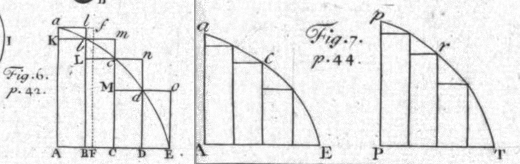
\includegraphics[scale=0.7]{img/newtons-fig.png}
	\caption{Newton's Motivating Figures for Lemma II}
	\tiny{Philosophiæ Naturalis Principia Mathematica, CC0}
\end{figure}

Newton observed that as he decreased the width of the rectangles, thus increasing
the quantity, he could get a better and better estimate of the true area. He
summarized this idea in a theorem he called Lemma II. 

\textbf{A Note About Reading Historical Math Texts:} Before going over this 
theorem it is important to note the difficulty of historical 
mathematical texts. In many cases, the difficulty of these texts does not always
originate from the mathematical content. Due to the lack of standardization of notation
and antiquated writing styles, older math texts can be difficult to parse. \cite{bourne:2010}.
Newton in particular was known for using obscure and difficult notation which made 
his work hard to interpret despite its brilliance. 
\begin{enumerate}
	\item In Old English, the symbol we use for integration today ($\int$) was 
		analogous to the letter $S$. For example, where we would write Sum, Newton 
		would write $\int$um. 	
	\item Another convention in older texts is the symbol \textit{\&c} which means 
		etc. or et cetera. In fact, \textit{et} is Latin for and, so the use
		of the ampersand is quite intuitive.
	\item Finally, Newton, among other mathematicians, frequently used the
		Latin phrase \textit{ad infinitum} or just \textit{infinitum} which means
		to infinity or infinitely. This phrase was invoked often to represent the idea
		of a limit or the repetition of some process to infinity. 
\end{enumerate}
We will see these conventions appear again when we look at the work of other early
mathematical work. 

\begin{lemma}\cite[Lemma II]{newton:}
	If any figure AacE (Pl.I.Fig6.) terminated by the right lines A a, AE, and 
	the curve AcE, there be in$\int$scrib'd any number of parallelograms A b, 
	B c, C d, \&c. comprehended under equal b$\int$es A B,B C, C D, \&c. and the 
	$\int$ides B b, C c, D d, \&c. parallel to one $\int$ide A a of the figure; 
	and the parallelogram a K b l, b L c m, c M d n, \&c are completed. Then if 
	the breadth of tho$\int$e parallelograms be $\int$uppos'd to be 
	dimini$\int$ed, and their number to be augmented in infinitum: I $\int$ay 
	that the ultimate ratio's which the in$\int$crib'd figure A K b L c M d D, 
	the circum$\int$scrib'd figure A a l b c n do E, and curvilinear figure 
	A a b c d E, will have to one another, are ratio's of equality. 
\end{lemma}
In more modern language, Newton is saying that as the number of rectangles 
increases and their width decreases, the ratio between their sums of the upper
and lower sums will get closer to 1 (or in other words produce an equal sum). 
Already in these early conceptions of the integral, we see glimpses of more 
rigorous definitions of the integral introduced first by Cauchy,
improved by Riemann, and further expanded upon by Lebesgue.

\subsection{Cauchy's Integral}

Augustin-Louis Cauchy (1789-1857) was a prolific mathematician of the $19^{th}$ century. 
Aside from this many specific mathematical contributions, Cauchy's goal was 
to develop a rigours analysis, and of course, this included the integral. 
The ideas of Newton and Leibniz provided a foundation for integration, but Cauchy
understood that their early conceptions still lacked rigor. 

In his text \textit{Summary of some Lessons on the Infinitesimal 
Calculus}\footnote{Résumé des Leçons sur Le Calcul Infinitésimal}, Cauchy 
introduces what he calls the definite  integral of a function $f(x)$. His
approach is similar to Leibniz and Newton in that he opts to partition the function's
domain and estimate the area with an infinite sum of rectangles. He writes, 
\begin{multicols}{2}
\begin{quote}
	Si l'on divise $X - x_0$ en élémens infiniment petits $x_1-x_0,
	x_2-x_1,\cdots X-x_{n-1}$, la somme 
	\begin{equation*}
	\begin{split}
		S&=(x_1-x_0 f)(x_0)+(x_1-x_2)f(x_1) + \cdots \\
		 & +(X-x_{n-1})f(x_{n-1})
	\end{split}
	\end{equation*}
	convergera vers une limite représentée par l'intégrale définie
	\begin{equation*}
		\int^X_{x_0} f(x) dx.
	\end{equation*}
\end{quote}
\begin{quote}
	If we divide $X - x_0$ into infinitely small elements,
	$x_1 - x_0,x_2 - x_1, \ldots, X - x_{n-1}$, the sum
	\begin{equation*}
	\begin{split}
		S &= (x_1 - x_0)f(x_0)+(x_2-x_1)f(x_1) + \ldots \\
		&+(X- x_{n-1})f(x_{n-1})
	\end{split}
	\end{equation*}
	will converge towards a limit represented by the definite integral
	\begin{equation*}
		\int^{X}_{x_0} f(x) dx.
	\end{equation*}
\end{quote}
\end{multicols}

In this first conception, Cauchy only looks at left hand (lower) rectangles in his 
construction. Additionally, he does not specify that each rectangle have an 
equal base. In other words $x_i - x_{i-1}$ need not equal $x_j - x_{j-1}$
\cite{gillespie:1915}. It is important to  note that, Cauchy only considered
functions that were continuous on $[x_0,X]$. More exotic discontinuous functions 
were of less interest at this time (if even fully understood). Additionally, 
without comment, he implies that  the length of the largest subinterval of the domain approaches $0$
\cite{kline:1972}. Many early math texts often assumed the reader would figure
out key details or took them as obvious. 

Later, Cauchy gave a more precise definition his integral where he allowed the
height of the rectangles to vary. Instead of fixing the height of each rectangle to
strictly be the image the left endpoint of each subinterval, he assigns a new 
variable $\zeta_i$ to be some random element from each subinterval and allows 
its image be the height of the rectangle \cite{cauchy:1823}. 
In more modern notation, we define Cauchy's definite integral as follows:
\begin{equation*}
	\int^{X}_{x_0} f(x) dx = \lim_{n\rightarrow \infty} \sum^{n}_{i=1}
	f(\zeta_i)(x_i - x_{i-1}).
\end{equation*}
This construction allowed Cauchy to define the integral arithmetically as
opposed the more loose geometric definitions that proceeded it. 

\subsection{Riemann's Integral}

Georg Frierdrich Bernhard Riemann (1826-1866) was one of the most famous
mathematicians from the $19^{th}$ century for his contributions to analysis and
number theory. Interestingly, even though Riemann's
integral is one of the most ubiquitous definitions of integration, it was 
more-or-less a footnote in his 1854 paper, \textit{On the representability of a function by 
trigonometric series}\footnote{Über die Darstellbarkeit einer Function durch eine 
trigonometrische Reihe}. Riemann developed his integral to be able to calculate
coefficients in infinite trigonometric series. Riemann needed a definition of 
integration that could handle functions with many discontinuities and developed 
it based on Cauchy's work earlier that century. In fact, Riemann's integral is 
equivalent to Cuachy's, but his is far more rigorously defined.

We will proceed with a modern definition of Riemann's integral in order to 
more easily demonstrate its strengths and limitations. We will begin
by setting up some standard definitions.

\begin{definition}
	A partition of an interval $[a,b]$ is defined as a finite sequence of real
	numbers such that:
	\begin{equation}
		a = x_0 < x_1 < x_2 < \ldots < x_n = b.
	\end{equation}
\end{definition}
\begin{definition}
	We define the length (or difference) of a subinterval of a partition as 
	$\forall i \in \{1,2,\ldots, n\}$:
	\begin{equation}
		\Delta x_i = x_i - x_{i-1}.
	\end{equation}
\end{definition}

\begin{definition}
	We define the mesh (or norm) of a partition $a = x_0 < x_1 <\ldots<x_n = b$ 
	of the interval $[a,b]$  as:
	\begin{equation}
		\max \Delta x \coloneqq \max\{|\Delta x_i|: i=1,\ldots,n \}.
	\end{equation}
\end{definition}

\begin{definition}
	Let $a = x_0 < \ldots < x_n = b$ be a partition of the interval $[a,b]$. We
	say $t_0,\ldots, t_{n-1}$ is a tagged partition if $\forall i \in \{1,2,.\ldots,n\}$:
	\begin{equation}
		x_i \leq t_i \leq x_{i+1}.
	\end{equation}
\end{definition}

The following definition is commonly referred to as the Riemann integral.

\begin{definition}
	Let $f:\R\rightarrow \R$ be a bounded function defined on the interval $[a,b]$, and
	let $x$ be a partition of $[a,b]$. Choose points $t_i$ in $[x_{i-1}, x_i]$.
	We define the Riemann integral, if it exists, of $f$ from $a$ to $b$ as:
	\begin{equation}
		\int^b_a f(x)dx = \lim_{\max \Delta x \rightarrow 0} 
		\sum^{n}_{i=1} f(t_i)(\Delta x_i ).
	\end{equation}
\end{definition}

From this definition, Riemann also gives us a criteria for integrability. 
In his original paper, Riemann defines upper and lower sums as follows. First, 
for any of the subintervals in the partition, he lets $M_i \coloneqq \max f([x_{i-1},x_i])$ and 
$m_i \coloneqq \min f([x_{i-1},x_i])$. We then have that the upper and lower
sums respectively:
\begin{equation*}
	S \coloneqq \sum^{n}_{i=1} M_i \Delta x_i, 
	 s \coloneqq \sum^{n}_{i=1} m_i \Delta x_i.
\end{equation*}

He defines $D_i \coloneqq M_i - m_i$ (this will always be positive by 
construction). He states that the integral of a function $f(x)$ exists if and 
only if the following condition holds:
\begin{equation*}
	\lim_{\max \Delta x \rightarrow 0} \sum^{n}_{i=1} D_i\Delta x_i = 0.
\end{equation*}
In other words, as the mesh of the partition tends towards $0$, the upper and 
lower sums will become closer and closer in size eventually cancelling each other
out. If the area of the rectangles do not get closer together in area, then 
we cannot take the integral.

\subsection{Limitations of Riemann's Integral} \label{sec:nonrie}

For most students, especially first year calculus students, the Riemann integral 
takes center stage as a highly intuitive and natural approach to integration, 
but we will soon see that although the Riemann integral is an incredibly 
powerful tool, it has many shortcomings which prove problematic for a
generalized theory of integration.

\subsubsection{Non-Riemann Integrable Functions}

The first limitation of the Riemann integral is the existence of bounded
functions whose Riemann integral is not defined. We begin with a standard 
example to demonstrate this. Let us define an indicator function on the
rational numbers, $\Q$. We define 
$1_{\Q}:\R \rightarrow \{0,1\}$ as,
\begin{equation*}
	1_{\Q} = \begin{cases}
		1 & x\in \Q  \\
		0 & x \in \R\setminus \Q \\
	\end{cases}.
\end{equation*}
This function was first introduced by  Johann Peter Gustav Lejeune Dirichlet
(1805-1859) in 1829, and while it feels quite artificial, it serves as a
useful counterexample. By the density of the irrationals in $\R$, it is clear 
that this function is highly discontinuous. We will see that this ``amount'' of discontinuities is enough to 
make this simple function non-Riemann integrable. Let's show this using 
Riemann's criteria.

\begin{prop}
	$1_{\Q}:[0,1] \rightarrow \{0,1\}$ is \textbf{not} Riemann integrable.
\end{prop}
\begin{proof}
	Let $0 = x_0 < x_1 <\cdots < x_n = 1$ be a partition of $[0,1]$ such that
	length of each subinterval of our partition is of equal size:
	\begin{equation*}
		\Delta x = \frac{1-0}{n}.
	\end{equation*}
	It suffices to show that $\lim_{\max \Delta \rightarrow 0}\sum^n_{i=1} D_i \Delta x_i \neq 0$.
	We observe that $\Q \cap [0,1]$ and $(\Q\setminus \R) \cap [0,1]$ are both
	dense in $[0,1]$. Thus every subinterval in our partition will contain 
	elements both from $\Q \cap [0,1]$ and $(\Q\setminus \R) \cap [0,1]$.
	This gives us that $\forall i, M_i =\max 1_{\Q}([x_{i-1},x_i]) = 1$ and 
	that $m_i = \min 1_{\Q}([x_{i-1},x_i]) = 0$. Thus we have 
	$\forall i, D_i = M_i - m_i = 1$. Taking our sum gives us:
	\begin{equation*}
		\begin{split}
			\lim_{\max \Delta x \rightarrow 0}\sum^n_{i=1} D_i \Delta x_i&=
			\lim_{n \rightarrow \infty}\sum^n_{i=1} \frac{i}{n}\\
			&= \lim_{n \rightarrow \infty}\frac{1}{n}\sum^n_{i=1} i\\
			&= \lim_{n \rightarrow \infty} \frac{n(n+1)}{2n}\\
			&= \lim_{n \rightarrow \infty} \frac{n + 1}{2}.\\
		\end{split}
	\end{equation*}
Thus our series diverges.
\end{proof}

\subsubsection{The Limit Problem} \label{sec:limitproblem}

The second major issue with the Riemann integral is often referred to as the 
limit problem \cite{loya}. Suppose we have a sequence of Riemann integrable bounded functions 
$f_n:[a,b] \rightarrow \R$ that converge to some bounded function 
$f:[a,b] \rightarrow \R$ does the following property always hold:
\begin{equation*} 
	\int^{b}_{a} f(x) dx = \lim_{n\rightarrow \infty} \int^{b}_{a} f_n(x)dx ?
\end{equation*}
We might expect this property to hold, but it does not. There are cases where 
the limit of a sequence of Riemann integrable functions is not a Riemann 
integrable function! In 1898, french mathematician René-Louis Baire (1874-1932) 
introduced a fairly innocent sequence of functions. Suppose that we define 
$\forall n \in \N, f_n:[0,1] \rightarrow \{0,1\}$ as:
\begin{equation*}
	f_n(x) = \begin{cases}
		1 & \text{if $x = p/q$ is rational in lowest terms with $q\leq n$}	\\
		0 & \text{otherwise }
	\end{cases}.
\end{equation*}

Let us look at an example. Suppose $n=4$, this gives us the following function:
\begin{equation*}
	f_4(x) = \begin{cases}
		1 & \text{if $x \in \{0,\frac{1}{4},\frac{1}{3},\frac{1}{2},\frac{2}{3},\frac{3}{4},1\}$ }	\\
		0 & \text{otherwise }
	\end{cases}.
\end{equation*}
We also have that given an $n \in \N$, $f_n$ is Riemann integrable. 
Let's use $f_2$ as an example. We have finite discontinuities at 
$\{0,\frac{1}{2},1\}$. Taking improper  Riemann integrals gives us:
\begin{equation*}
	\begin{split}
	\int^{1}_{0} f_2(x)dx &= 
			\lim_{t\rightarrow 0^+} \int^{\frac{1}{4}}_{t} f_2(x) dx +
 			\lim_{t\rightarrow \frac{1}{2}^-} \int^t_{\frac{1}{4}} f_2(x) dx +
 			\lim_{t\rightarrow \frac{1}{2}^+} \int^{\frac{3}{4}}_t f_2(x) dx +
 			\lim_{t\rightarrow 1^-} \int^t_{\frac{3}{4}} f_2(x) dx \\
			&= 0 + 0 + 0 + 0 = 0.
	\end{split}
\end{equation*}
We see that this generalizes given any value $n\in \N$, $f_n$ will have a
Riemann integral of value $0$. Thus every $f_n$ in our sequence is Riemann
integrable. However, observe what happens when we take the limit of $f_n$.
$\forall x \in [0,1]$, we have:
\begin{equation*}
	\lim_{n\rightarrow \infty} f_n(x) = 
	\begin{cases}
		1 & \text{if $x \in \Q$} \\
		0 & \text{otherwise } \\
	\end{cases}
	= 1_{\Q}(x).
\end{equation*}
Therefore there is a possibility that a sequence of Riemann integrable 
functions can converge to a nonintegrable function.

\subsubsection{The Anti-Derivative Problem} \label{sec:antiderivativeproblem}

There is another issue with the Riemann integral relating to the fundamental
theorem of calculus (FTC). For some time, the following
statement was taken as fact.

Let $f:[a,b] \rightarrow \R$ be a  bounded function on $[a,b]$ and $F$ be the 
anti-derivative of $f$ such that $\forall x \in [a,b], F'(x) = f(x)$. Then the
following equality holds.
\begin{equation*}
	\int^{b}_{a} f(x) dx = F(b) - F(a).
\end{equation*}
However, if the integral in the above equality is the Riemann integral, 
this equality does not always hold. That is, we can show that there exists a 
bounded, continuous, real-valued function $F$ on $[a,b]$ whose derivative $f$ exists, 
yet $\int^{b}_{a}f(x)$ is not defined in terms of Riemann. Such a function was described by 
Italian mathematician Vito Volterra (1860-1940) in 1881, but it requires some 
more theory to set up which will will discuss in a later section. For now, know 
that this is a limitation of the Riemann integral.

\subsection{Summary}

From the $16^{th}$ to $19^{th}$ century, the mathematical community developed a 
more rigorous definition of the definite integral based on the properties of 
infinite sums. These integrals all relied on partitioning 
the domain of a function. They were able to integrate both continuous functions 
and functions with jump discontinuities. However, this definition of the
integral had some severe limitations that motivated future development of the 
theory of integration and raised the following questions:
\begin{enumerate}
	\item Can we develop a more inclusive integral to handle highly
		discontinuous functions?
	\item How discontinuous can a function be  before it can no longer be 
		Riemann integrable?
	\item Can we fix fundamental theorem of calculus?
\end{enumerate}
French mathematician Henri Lebesgue (1875-1941) saw these issues and 
came up with a novel solution that changed the theory of integration in a revolutionary way. In 
his ground breaking paper \textit{On a generalization of the definite integral},
\footnote{Sur une généralisation de l'intérale définie} Lebesgue writes,
``Riemann defined the integral of certain discontinuous functions, but all 
derivatives are not integrable in the sense of Riemann. Research into the
the problem of anti-derivatives is thus not solved by integration, and one can
desire a definition of the integral$\ldots$allowing one to solve the problem of
anti-derivatives \cite{lebesgue:1901}.'' It is important to keep in mind that 
this was Lebesgue's primary motivator when exploring integration. Like Newton, 
his approach was to treat integral as an inverse of differentiation.

\section{Measure Theory}

In order to discuss Lebesgue's integral, we need to set up some important
tools--particularly a general theory of measure on sets. Measure theory is the 
foundation of Lebesgue's theory of integration, and it requires much discussion.
Before jumping into the theory of measure in $\R$ we briefly need to set up some new
notation. 
\begin{definition}
	We define the extended real numbers as the following set:
	\begin{equation}
		\bar{\R} \coloneqq \R \cup \{-\infty,\infty\}.
	\end{equation}
\end{definition}
In the extended real numbers, we treat $\pm\infty$ as a valid mathematical object
that sits on the line of extended real numbers. Keeping this concept in mind, 
in the most abstract sense, a measure is a mapping from a given set to some value in 
the extended real number line. The notation of the extended reals allows a set
to have measure $\infty$ or $-\infty$.
\begin{equation*}
	m: \sM \rightarrow \bar \R.
\end{equation*}

\subsection{Measure in $\R$}

While most modern applications measure theory are concerned with more abstract spaces,
historically, Lebesgue and other measure theorists began by investigating
measure on line and the plane. Since we are approaching Lebesgue's theory of 
integration from a historical perspective, we will begin on the line.

In his 1902 paper titled \textit{Integral, Length, Area}\footnote{Intégrale, 
Longueur, Aire} \cite{lebesgue:1902}, Lebesgue outlined 
the following conditions for his measure. He wrote,
\begin{multicols}{2}
\begin{quote}
	Nous nous proposons d'attacher à chaque ensemble borné un nombre positif ou
	nul que nous appellerons sa mesure et satisfaisant aux conditions suivantes:
	\begin{enumerate}
		\item Il existe des ensembles dont la mesure n'est pas nulle.
		\item Deux ensembles égaux ont même mesure.
		\item La mesure de la somme d'un nombre fini out d'une infinité
		dénombrable d'ensembles, sans points communs, deux à deux, est la somme
		des mesures de ces ensembles.
	\end{enumerate}
\end{quote}

\begin{quote}
	We propose to attach a positive number or zero to each bounded set that we 
	call its measure and satisfies the following conditions:
	\begin{enumerate}
		\item There exists sets that have a non-zero measure.
		\item Two sets that are equal have the same measure.
		\item The measure of the sum of a finite or a denumerable [countablely] infinite number
		 of sets without points in common, pairwise disjoint, is the sum of
		 measures of these sets.	
	\end{enumerate}
\end{quote}
\end{multicols}

In more modern notation, we define such a measure as the \textit{Lebesgue measure}.
Let us introduce a measure and see if it satisfies Lebesgue's criteria.
We will by defining the length of an interval. 
\begin{definition}
	Let $I \subset \R$ be an interval with endpoints $a \leq b$. We define
	the length of $I$ as:
	\begin{equation}
		|I| \coloneqq b - a.
	\end{equation}
\end{definition}

From this simple definition we elect the following measure as a candidate to 
satisfy the criteria for Lebesgue's measure.
\begin{definition}
	Let $A \subseteq \R$. We define the \textit{outer measure} of $A$ as:
	\begin{equation}
		m^*(A) \coloneqq \inf \bigg\{ \sum_{k=1}^{\infty} |I_k| : \textit{ $(I_k)^\infty_{k=1}$ is a sequence of
		open intervals with $A \subseteq \bigcup_{k=1}^{\infty}I_k$ } \bigg\}.
	\end{equation}
\end{definition}

Before moving on, we will outline some important properties of the outer
measure so that we can become more comfortable using it. First we will show 
that the outer measure of a closed interval is just its length.
\begin{theorem}
	Given any closed and bounded interval $A \subset \R$ with endpoints $a\leq b$, 
	then $m^*(A) = |A|$.
\end{theorem}
\begin{proof}
	It suffices to show that $m^*(A) \leq |A|$ and $m^*(A) \geq |A|$.
	\begin{enumerate}
	\item 
		We want to show $m^*(A) \leq |A|$. Let $\epsilon > 0$ be given. 
		Define an open covering of $A$ as $\forall k \in \N$:
		\begin{equation*}
			I_k = \begin{cases}
				(a-\frac{\epsilon}{2}, b+\frac{\epsilon}{2}) & k = 1\\
				\emptyset &  k > 1. \\
		\end{cases}
		\end{equation*}
		Taking the outer measure of $\bigcup_{k=1}^{\infty}$ gives us:
		\begin{equation*}
			m^*(A) \leq \big(b+\frac{\epsilon}{2}\big) - \big(a-\frac{\epsilon}{2}\big) = b-a+\epsilon. 
		\end{equation*}
		Therefore we have $m^*(A) \leq b-a = |A|$ as required.
	\item We want to show that $m^*(A) \geq |A|$. Let $a$ be the left endpoint of
		$A$ and $b$ be the right such that $a \leq b$. Let $(I_k)^{\infty}_{k=1}$ be
		some open cover of $A$.	Since $A$ is an interval, then it is compact. 
		Thus, we can choose a finite subcover of $A$. Let us enumerate our finite 
		covering $I_1,I_2,\cdots,I_N$ such that $a \in I_1$ and $b \in I_N$ 
		(provided that $b\neq a$ otherwise, $b\in I_1$). This gives us:
		\begin{equation*}
			a = a_1 < a_2 < \cdots < a_{N+1} = b, (a_j,a_{j+1}) \subseteq I_{j}.
		\end{equation*}
		Taking the infimum over all possible finite subcovers gives us:
		\begin{equation*}
			|A| = b - a = a_{N+1} - a_1 = \sum^{N}_{j=1} a_{j+1} - a_{j} \leq 
			\sum_{j=1}^{N} |I_j| \leq \sum_{j=1}^{\infty} |I_j|.
		\end{equation*}
		Therefore $m^*(A) \geq |A|$.
	\end{enumerate}
\end{proof}

The proof for open and half open intervals is similar which yields the following
theorem.
\begin{theorem}
	Let $I \subseteq \R$ be an interval, then $m^*(I) = |I|$.
\end{theorem}

Additionally, this theorem shows that this outer measure satisfies Lebesgue's 
first criteria for a measure. Take the unit  interval $m^*([0,1]) = 1$. 
Thus, there exists a set without measure $0$. Additionally, because of
uniqueness of infimum, two equal sets will have the same outer measure
satisfying the second condition.  Next, we will show that all 
countable sets have a measure of $0$. 
\begin{theorem}
	Let $A$ be a countable set, then $m^*(A) = 0$.
\end{theorem}
\begin{proof}
	It suffices to show that $\forall \epsilon > 0, m^*(A) \leq \epsilon$.
	Let $\epsilon > 0$ be given, enumerate the elements of $A$ as 
	$(x_k)^{\infty}_{k=1}$, and let $I_k$ be an open interval of length 
	$\epsilon/2^k$ that contains $x_k$. Then we have that the collection 
	$\{I_k\}$ covers $A$. This gives us: 
	\begin{equation*}
		\begin{split}
			m^*(A) \leq \sum_{k=1}^{\infty} |I_k| &= \sum_{k=1}^{\infty} \frac{\epsilon}{2^k}  \\
					&= \sum_{k=1}^{\infty} \epsilon \bigg(\frac{1}{2}\bigg)^k  \\
					&= \epsilon \bigg(\frac{1/2}{1-1/2}\bigg)  \\
					&= \epsilon. \\
		\end{split}
	\end{equation*}
\end{proof}

These theorems yield the following properties of the outer measure.
\begin{theorem} \label{thm:mprop}
	The following properties of the outer measure hold. 
	\begin{enumerate}
		\item $0 \leq m^*(A) \leq +\infty$;
		\item $A\subseteq B \implies  m^*(A) \leq m^*(B)$;
		\item $A\subseteq \bigcup^{\infty}_{k=1} A_k \implies m^*(A) \leq
			\sum^{\infty}_{k=1}m^*(A_k)$;
		\item Let $A$ be an interval, then $m^*(A) = |A|$;
		\item $m^*(A+h) = m^*(A)$.
	\end{enumerate}
\end{theorem}

\subsection{Measureability in $\R$}

As we have been working with the outer measure, the reader will note that we 
have demonstrated the outer measure satisfies Lebesgue's first two criteria 
for a measure, but we have have thus far been silent on the third criteria. 
Rewriting Lebesgue's third requirement in modern notation, we would expect that 
given any countable collection of pairwise disjoint  sets $\{C_k\}$,
\begin{equation*}
	m^*(C_0 \sqcup C_1 \sqcup \ldots \sqcup C_k \sqcup \ldots ) =  
	m^*(C_0)+m^*(C_1)+ \ldots + m^*(C_k) + \ldots 
\end{equation*}
This only seems natural. The next question is: does this work for every
subset of the real line? As surprising as it is, the answer is no. Will see 
in a later section that Italian mathematician Giuseppe Vitali (1875-1932) 
demonstrated that, in fact, not all sets of the real line satisfy this property.  
If we try to measure a set that does \textit{not} have this property, then the measure 
of such a set would be of little use to us. In order to account for the fact 
that not all sets conform to this criteria, we simply restrict the sets that we 
that we can measure. 

This was no surprise to Lebesgue. Returning to his work \textit{Integral, Length,
and Area}\cite{lebesgue:1902}, he commented heavily on the possibility of nonmeasurable sets. He 
referred to this issue generally as, \textit{the problem of measure}. In fact, 
Lebesgue outlined a criteria of measureability that he ad adapted from the
work of mathematician Émile Borel (1871-1956) who also made major contributions
to measure theory. Lebesgue states,
\begin{multicols}{2}
\begin{quote}
	Nous ne résoudrons ce \textit{problème de la mesure} que pour les ensembles
	que nous appellerons mesurables$\ldots$Nous appellerons \textit{ensembles 
	mesurables ceux dont les mesures extieure et intérieure sont égales}, la
	valeur commune de ces deux nombres sera la mesure de l'ensemble, problème 
	de la mesure est possible. 
\end{quote}
\begin{quote}
	We will [only] solve this \textit{problem of measure} for sets that we call
	measurable$\ldots$We will call \textit{measurable sets those whose
	exterior measure and interior measure are equal}. The value in common between
	these two numbers will be the measure of the set, if the problem of measure is 
	possible. 
\end{quote}
\end{multicols}
Today, we still use this concept of measureability in a more concise form. The
following is the modern definition of measureability.
\begin{definition}
	Let $A \subseteq \R$. $A$ is said to be measurable if, $\forall E\subseteq \R,$
	\begin{equation}
		m^*(E) = m^*(E\cap A)+m^*(E\cap A^c).
	\end{equation}
\end{definition}

Abiding by this restriction, it is useful to define a superset that contains all
the sets which Lebesgue deemed measurable.
\begin{definition}
	We denote $\sM$ as the set of all measurable sets. 
\end{definition}
The next theorem shows that, because of the subadditivity of the outer measure,
we can obtain a lighter condition for measureability.  
\begin{theorem}
	Let $A\subseteq \R, \forall E \subset \R, m^*(E) \geq m^*(E\cap A) + m^*(E\cap A^c) \implies A \in\sM$ 
\end{theorem}
\begin{proof}
	Let $E \subseteq \R$ be given. Observe that $E = (E\cap A) \cup (E\cap A^c)$. 
	By subadditivity we have:
	\begin{equation*} 
		m^*(E) = m^*((E\cap A) \cup (E\cap A^c)) \leq  m^*(E\cap A) + m^*(E\cap A^c).
	\end{equation*}
	Thus by definition of measurability, it suffices to prove show that 
	$m^*(E) \geq m^*(E\cap A) + m^*(E\cap A^c)$.
\end{proof}

The following theorem shows that all sets of measure $0$ are measurable. 
\begin{theorem} \label{thm:zerosets}
	Let $A\subseteq \R, m^*(A) = 0 \implies A \in \sM$.
\end{theorem}
\begin{proof}
	Let $E\subseteq \R$ be given. We observe that $E\cap A \subseteq A$, thus
	we have that: 
	\begin{equation*}
		0\leq m^*(E\cap A) \leq m^*(A) = 0.
	\end{equation*}
	We also have that $A^c \cap E \subseteq E$ which gives us $m^*(A^c\cap E) \leq m^*(E)$.
	Thus we have:
	\begin{equation*}
		m^*(E\cap A) +m^*(E\cap A^c) \leq m^*(E).
	\end{equation*}
\end{proof}

An additional property is that, if a set is measurable, then its complement is
also measurable. This follows directly from the definition of measureability.
\begin{theorem} \label{thm:complement}
	$A \in \sM \implies A^c \in \sM$.
\end{theorem}
\begin{proof}
	Let $E$ be given. Since $A \in \sM$, we have:
	\begin{equation}
		m^*(E) = m^*(E\cap A) +m^*(E\cap A^c) =  m^*(E\cap A^c) +m^*(E\cap A).
	\end{equation}
\end{proof}

The next theorem will prove that if a collection of disjoint sets are each
measurable, then the outer measure will satisfy Lebesgue's third condition 
for measure. First we will need to prove a lemma.

\begin{lemma} \label{lemma:ctlbadd}
	Let $\{A_N\}$ be a countable collection of pairwise disjoint and measurable 
	sets. Let $E \subset \R$. Then the following holds:
	\begin{equation}
		m^*\bigg( E\cap \bigcup_{k=1}^N  A_k \bigg) = \sum_{k=1}^N m^*(E\cap A_k).
	\end{equation}
\end{lemma}
\begin{proof}
	The base case $N=1$ is trivial.
	For $1\leq n \leq N$, let $B_n = \bigcup_{k=1}^n A_k$. By induction,
	assume that,
	\begin{equation*}
		m^*(E \cap B_n) = \sum_{k=1}^n m^*(E\cap A_k).
	\end{equation*}
	Applying our induction hypothesis gives the following,
	\begin{equation*}
		\begin{split}
		m^*(E\cap B_{n+1}) &= m^*(E\cap A^c_{n+1} \cap B_{n+1}) + m^*(E\cap A_{n+1} \cap B_{n+1})  \\
			&= m^*(E\cap B_{n}) + m^*(E \cap A_{n+1}) \\
			&= \sum_{k=1}^n m^*(E\cap A_{k}) + m^*(E \cap A_{n+1}). 
		\end{split}
	\end{equation*}
\end{proof}
\begin{theorem} \label{thm:union}
	Let $(A_k)^{\infty}_{k=1}$ be a sequence of pairwise disjoint and 
	measurable sets, then $\bigcup^{\infty}_{k=1}A_k$ is measurable and
	\begin{equation}
		m^*\bigg(\bigcup^{\infty}_{k=1} A_k \bigg) = \sum^{\infty}_{k=1} m^*(A_k).
	\end{equation}
\end{theorem}
\begin{proof}
	We want to show that $\bigcup^{\infty}_{k=1}A_k$ is measurable and 
	$m^*\bigg(\bigcup^{\infty}_{k=1} A_k \bigg) = \sum^{\infty}_{k=1} m^*(A_k)$.
	\begin{enumerate}
		\item Let $E \subset \R$ be given. Let $B_n = \cup^{n}_{k=1} A_k$ and 
		$B = \cup^{\infty}_{k=1}$. Since $B_n$ is measurable, by lemma \ref{lemma:ctlbadd},
		\begin{equation*}
			m^*(E) = m^*(E \cap B_n) + m^*(E\cap B^c_n) = 
			\bigg(\sum^n_{n=1} m^*(E\cap A_n)\bigg) + m^*(E\cap B^c_n). 
		\end{equation*}
		Since $B^c \subseteq B^c_n$, we can take the limit as $n\rightarrow\infty$ 
		giving us,
		\begin{equation*}
			m^*(E) \geq \bigg( \sum^{\infty}_{k=1} m^*(E\cap A_k) \bigg) +
			m^*(E \cap B^c) \geq m^*(E\cap B)+m^*(E\cap B^c).
		\end{equation*}
		Therefore $B = \bigcup^{\infty}_{n=1} A_n$ is measurable. We also have
		that,
		\begin{equation*}
			m^*(E) = m^*(E\cap B) + m^*(E\cap B^c) \leq 
			\bigg(\sum^{\infty}_{n=1}m^*(E\cap A_n) \bigg) + m^*(E\cap B^c)
		\end{equation*}
		\item  Now, we want to show that this sum is additive. From above, we
		have the following equality, 
		\begin{equation*} 
			m^*(E) = \sum^{\infty}_{k=1} m^*(E\cap A_k) + 
			m^*\bigg( E \cap \bigg(\bigcup^{\infty}_k A_k\bigg)^c\bigg) 
		\end{equation*} 
		Since $E$ was taken to be arbitrary, let $E = \bigcup^{\infty}_k A_k $.
		This gives us,
		\begin{equation*} 
			m^*\bigg(\bigcup^{\infty}_{k=1} A_k \bigg) = \sum^{\infty}_{k=1} m^*(A_k). 
		\end{equation*} 
	\end{enumerate}
\end{proof}

From this, it follows the infinite intersection of a sequence of measurable sets is also measurable.
This fact will prove useful in later sections.
\begin{theorem} \label{thm:intersection}
	Let $(A_k)^{\infty}_{k=1}$ be a sequence of pairwise disjoint measurable sets. Then
	$\bigcap^{\infty}_{k=1} A_k$ is also measurable.
\end{theorem}
\begin{proof}
	We have:
	\begin{equation*}
		\bigcap^{\infty}_{k=1} A_k = \bigg(\bigcup^{\infty}_{k=1}A^c_k\bigg)^c.
	\end{equation*}
	By theorem \ref{thm:complement}, since each $A_k$ is measurable, then
	$A^c_k$ is also measurable, so applying theorem \ref{thm:union} we have that 
	$\bigcup^{\infty}_{k=1}A^c_k$ is measurable. Finally, we apply theorem 
	\ref{thm:complement} again, and conclude $\bigcap^{\infty}_{k=1} A_k$ is
	measurable. 
\end{proof}

Now that we have shown that the outer measure satisfies Lebesgue's
three criteria under the constraint of measureability we can finally define 
the Lebesgue  measure.
\begin{definition}
	Let $A\subseteq \R$ be measurable, then its \textit{Lebesgue measure} is:
	\begin{equation}
		m(A) \coloneqq m^*(A).
	\end{equation}
\end{definition}
At this point, it should be clear why the Lebesgue measure is a powerful tool.
Many of the basic sets that we would expect to be measurable are. However, we 
still have the question of whether or not nonmeasurable sets exist. 

\subsection{A Nonmeasurable Set}
\begin{quote}
	\textit{The problem of measuring sets of points of a straight line is
	insurmountable.}

	\uppercase{\tiny{- Giuseppe Vitali}}	
\end{quote}

As alluded to earlier, nonmeasurable sets exist. The existence of
such sets were of great concern to mathematicians at the turn of the $20^{th}$ century
as it called into question the utility of measure. In this next section, we will
give an example of a nonmeasurable set in addition to discussing the theoretical
considerations given its existence.

\subsubsection{A Nonmeasurable Construction in $\R$}

The first mathematician to construct a Lebesgue nonmeasurable set was Giuseppe 
Vitali in 1905 \cite{vitali:1905}. Vitali's construction relied on a clever use 
of the Axiom of Choice.  This move is subtle, but it is the crux of the argument. 
We will go over an example presented by Frank Burk in his book 
\textit{Lebesgue Measure and Integration: An Introduction} \cite{burk:1998},
as it provides far more detail than Vitali's original paper.

We begin by setting up an equivalence relation such that for any  $x,y \in \R, 
x \sim y$ if and only if the difference $x-y$ is rational. These give rise to 
the following equivalence classes:
\begin{equation*}
	E_{x} = \{ y \in \R : x-y \in \Q \}.
\end{equation*}
These equivalence classes have the following properties:
\begin{enumerate}
	\item $\R = \cup E_{x}$.
	\item $x_1 \sim x_2 \implies E_{x_1} = E_{x_2}$.
	\item $E_{x_1} \cap E_{x_2} \neq \emptyset \implies E_{x_1} = E_{x_2}$.
\end{enumerate}
Based on these properties we observe that we have created a valid partition of 
$\R$. Using this partition, we will create a nonmeasurable set of $\R$ contained in
the open interval $(-1,1)$. We begin by creating equivalence classes of the 
elements in $(-1,1)$ such that
\begin{equation*}
	(-1,1) \cap E_x = \{ y \in (-1,1) : x-y \in \Q \}.
\end{equation*}
We observe the following about the collection $\{E_x\}$:
\begin{enumerate}
	\item Each $E_x$ is countable;
	\item The entire collection of distinct sets $E_x$ is uncountable.
\end{enumerate}
Now, let us \textit{choose} one element from each $E_x$ such and place it in a new 
set $\sV$. This step is subtle, but we have just invoked the Axiom of Choice to 
construct this set. This will inevitably  lead to the nonmeasurability of this set.

\begin{prop}
	$\sV$ is nonmeasurable.
\end{prop}
\begin{proof}
	Assume towards contradiction that $\sV$ is measurable. Observe the following about $\sV$:
	\begin{enumerate}
		\item $\sV$ is uncountable.
		\item $\forall x \in (-1,1), \sV \cap E_x$ is a singleton.
	\end{enumerate}

	Next, let us enumerate the rational numbers in the open interval $(-2,2)$. Let
	us call this enumeration $(q_k)_{k=1}^{\infty}$. We define:
	\begin{equation*}
		\sV + q_i = \{ x + q_n : x \in \sV, q_i \in (q_k)_{k=1}^{\infty} \}.
	\end{equation*}
	We then observe the following containments:
	\begin{itemize}
		\item $(-1,1) \subseteq \cup \sV + q_k$;
		\item $\sV + q_i \subseteq (-3,3)$.
	\end{itemize}

	Thus we have that the collection of sets $\{\sV + q_n\}$ creates a countable
	and disjoint cover of $(-1,1)$. Thus we have:
	\begin{equation*}
		(-1,1) \subset \bigcup^{\infty}_{k=1} (\sV+q_k) \subset (-3,3).
	\end{equation*}
	The monotonicity of the outer measure measure gives us:
	\begin{equation*}
		m(-1,1) \leq m\bigg(\bigcup^{\infty}_{k=1} (\sV+q_k) \bigg) \leq m(-3,3).
	\end{equation*}
	The countable additivity of the outer measure gives us:
	\begin{equation*}
		m(-1,1) \leq \sum_{k=1}^{\infty} m(\sV+q_k) \leq m(-3,3).
	\end{equation*}
	Since each $\{\sV+q_k\}$ is a translate of $\sV$, then by (5) of theorem \ref{thm:mprop}, 
	we have that each $m(\sV+q_k) = m(\sV)$. Substitution gives us:
	\begin{equation*}
		m(-1,1) \leq \sum_{k=1}^{\infty} m(\sV) \leq m(-3,3).
	\end{equation*}
	Evaluating $m((-1,1)) = 2$ and $m((-3,3)) = 6$. Since $\sum_{k=1}^{\infty} m(\sV)
	\leq 6$, then $m(\sV) = 0$ because a infinite sum of a constant diverges to
	$\infty$. Since $2 \leq \sum_{k=1}^{\infty} m(\sV)$, then $m(\sV) > 0$. Thus
	we have a contradiction, and $\sV$ is nonmeasurable. 
\end{proof}

\subsubsection{An Analogy About Sawdust}

Now that we have seen that there exists a nonmeasuarable set, this raises a 
natural question: if there exists sets that 
are not measurable by the outer measure, then why not develop a better measure? 
This is a fair question because having a theory of measurement that cannot handle every 
set is concerning to some. Historically, many mathematicians have pushed against measure theory
because of the existence of such sets. This, of course, greatly over
looks the utility of measure which we will explore in later sections. 
It is important to note that a measurement is only as useful as its utility. 
The fact is, it is rare that we encounter unmeasurable sets. It is not 
impossible, as we have demonstrated above, but one can see that they are not 
obvious. 

To drive this point home, I will reference an analogy from my capstone
mentor. He said, ``you would use a ruler to measure a board, but it would be 
impractical to use a ruler to measure sawdust.'' Measure, like a ruler, is a 
tool that has practicality and great use in many circumstances even if it has 
constraints. Additionally, this does not mean we cannot ``measure'' sawdust, we 
simply need a different \textit{way} to measure it--take for example weight or 
volume. The same can be said for these nonmeasurable sets; their existence does 
not threaten the utility of measure theory. Instead, they demonstrate a context 
in which this particular measure would be a poor tool. 

The fact is, the outer measure is a \textit{very} practical measure. The
nonmeasurable sets in terms of Lebesgue are relatively rare and often only of
interest when demonstrating that they are not measurable. Additionally, the 
outer measure is a fairly intuitive measure. As we have seen, when working with
intervals it takes their lengths; it assigns a measure of $0$ to countable 
sets; it handles both simple and complex sets with relative ease; and it 
generalizes quite nicely. Fundamentally, the outer measure is a tool, and like 
all tools, it is incumbent on the user to know when it is appropriate to use it.

As a final word on this subject, we mentioned during the construction that this 
example relies on a clever use of the Axiom of Choice. A natural question might 
be: can we construct a nonmeasurable set without relying on the Axiom of Choice? 
As it turns out, it is not possible. In his 1970 paper 
\textit{A Model of Set-Theory in Which Every Set of Reals is 
Lebesgue Measurable}, mathematician Robert M. Solovay demonstrates that the only 
way to construct a nonmeasurable set in terms of Lebesgue is by use of the 
Axiom of Choice \cite{solovay:1970}. 

\section{A Lengthy Aside on Smith, Cantor, and Volterra}

Now that we have a notion of measure and measureability in $\R$, we will return 
to the Riemann integral to develop a better understanding of why Lebesgue was so 
interested in the anti-derivative problem.

After the introduction of the Riemann integral to the greater mathematical
community in 1868, the following decade saw mathematicians become increasingly 
interested in investigating the, ``conditions under which a function could be 
integrated \cite{fleron:1994}.'' Specifically, mathematicians spent a great
deal of time constructing functions with infinite discontinuities that were
still integrable in the sense of Riemann \cite{kline:1972}. This work gave
rise to a famous theorem called the Lebesgue Criterion for Riemann integrability
which gives us precise conditions under which a function can be integrated using 
Riemann's definition. The next theorem is the Lebesgue Criterion for Riemann
integration.
\begin{theorem}[Lebesgue Criterion for Riemann Integration]
	Let $f:[a,b] \rightarrow \R$, and let $D(f) \coloneqq \{x \in [a,b] : 
	\text{ f is discontinuous at x }\}$. We say that $f$ is Riemann integrable
	if and only if $f$ is bounded and $D(f)$ has Lebesgue measure $0$.
\end{theorem}
Before moving on, let's look at some examples to illustrate the necessity of the
hypotheses. Let us first return to the Dirichlet function. Clearly $1_{\Q}$ is
a bounded function, but from an earlier section, we know that it is not Riemann 
integrable, so what is its domain of discontinuity? We claim that 
$1_{\Q}$ is everywhere discontinuous.

\begin{prop}
$1_{\Q}:[0,1] \rightarrow \{0,1\}$ is nowhere continuous (everywhere discontinuous)
on $[0,1]$. 
\end{prop}
\begin{proof}
	Let $x \in [0,1]$ be given. We have exactly two cases (1) $x \in \Q \cap
	[0,1]$ or (2) $x \in [0,1]\setminus \Q$.
	\begin{enumerate}
		\item Assume that $x$ is rational. Choose $\epsilon = \frac{1}{2}$.
		Let $\delta > 0$ be given. By density of the irrationals in $\R$,
		choose an irrational number $y \in [0,1]$ such that $|x-y|<\delta$. 
		We have:
		\begin{equation*}
			|1_{\Q}(x) - 1_{\Q}(y)| = |1-0| =1>\frac{1}{2}.
		\end{equation*}
		\item Assume that $x$ is irrational. Again, choose $\epsilon =
		\frac{1}{2}$. Let $\delta > 0$ be given. By density of the rationals in
		$\R$, choose a rational number $y \in [0,1]$ such that $|x-y| < \delta$.
		We have:
		\begin{equation*}
			|1_{\Q}(x) - 1_{\Q}(y)| = |0-1| =1>\frac{1}{2}.
		\end{equation*}
	\end{enumerate}
\end{proof}
This fact tells us the set of discontinuities of $1_{\Q}$ on $[0,1]$ is $[0,1]$,
and since $[0,1]$ is an interval, then $m([0,1]) = 1 > 0$. Thus we cannot simply
have a bounded function.

The other hypothesis states that Riemann integral must be taken on a bounded
function. This was mentioned in the definition of the Riemann integral, but we
have not explored it in great detail. Here is another question, what would
happen if we tried to take the integral of the following function on the
interval $[0,1]$? 
\begin{equation}
	h(x) = \begin{cases}
		\frac{1}{x} & \text{if $x\neq 0$}\\
		0 & \text{otherwise} 
	\end{cases}.
\end{equation}
First, it is clear that on $[0,1]$ that $D(h) = \{0\}$  and as a result has measure 
$0$. Further more, it is obvious that $h$ is not bounded. We see that it approaches
$\infty$ as $x \rightarrow 0^-$. Thus we only have one hypothesis satisfied. 
We will show that this is not a sufficient condition for Riemann integrability.

Let us begin in our usual fashion by creating a partition of $[0,1]$ such that
$0 = x_1 < x_2 < \cdots < x_n = 1$. Suppose now that we want to find the height
of the right hand rectangles on this partition, we have that $\sup(h([0,x_1])) =
\infty$. Clearly we cannot interpret such a height. Thus we must have a bounded
function.

Now that we have briefly explored the necessity of the hypotheses in Lebesgue's
criteria, we will look at some historical motivating examples that led 
Lebesgue to become interested in the anti-derivative problem mentioned in
section \ref{sec:antiderivativeproblem}.

\subsection{Cantor Sets}

Historically, our conversation begins with Cantor sets. Cantor sets are
quite famous and appear in many fields of mathematics in novel and unexpected ways.
However, their discovery was directly related to  integration theory. 
While Cantor sets are most commonly associated with the mathematician Georg 
Cantor (1845-1918) who wrote about them in 1883, they were 
actually introduced in 1875 by Irish, Oxford professor, Henry John Stephen 
Smith (1826-1883) in his paper titled \textit{On the Integration of 
Discontinuous Functions}, and to this date, is
their earliest known mention. While Cantor's paper is much more famous, Smith's 
paper introduced a important idea in the development of understanding integrable 
functions \cite{scoville:2019}. At the time, Smith was relatively unknown
to the greater mathematical community, and his discoveries were not recognized 
until much later. In his work, Smith was interested in constructing sets whose points
he described as lying in \textit{loose order}. He wrote,
\begin{quote}
	A system of points is said to \textit{fill completely} a given interval, when any
	segment of the interval being taken, however small, one point at least of
	the system lies on that segment\ldots points are in close order on any
	segment when the completely fill it, and in \textit{loose order}, and
	in \textit{loose order} when they do not completely fill it or any pare of
	it, however small \cite{smith:1875}.
\end{quote}
The observant reader will note that when Smith talks about points who
\textit{fill and interval completely} he is discussing the concept of density.
Smith's concept of a system of \textit{loose order} order
points would be describe today as a \textit{nowhere dense set}.

The sets we have looked at up until this point have been fairly straight forward 
and easy to visualize (aside from $\sV$), but the measure of a nowhere dense set like the  
Cantor Set is not immediately obvious. While Smith was the first person to come 
up with a generalized Cantor set, Cantor's middle thirds set serves as a fairly straight 
forward introduction into  nowhere dense sets. In his famous paper titled 
\textit{On infinite linear manifolds of points, Part 5}, Cantor defined his set 
by beginning with the closed unit interval $[0,1]$ which we will denote $C_0$. 
Then he removes the middle third, and labels the union of the remaining
closed intervals $C_1$: 
\begin{equation*}
	C_1 = \bigg[0,\frac{1}{3}\bigg] \cup \bigg[\frac{2}{3},1\bigg].
\end{equation*}
Then, he continues this process for each smaller interval, so for example, 
to go from $C_1$ to $C_2$, we remove the middle thirds of the two intervals that
make up $C_1$. 
\begin{equation*}
	C_2 = \bigg[0,\frac{1}{9} \bigg] \cup \bigg[\frac{2}{9},\frac{1}{3}\bigg] 
	\cup \bigg[\frac{2}{3},\frac{7}{9}\bigg] \cup \bigg[\frac{8}{9},1\bigg].
\end{equation*}
As we continue this process to infinity, we observe the following relationship:
\begin{equation*}
	C_1 \supset C_2 \supset C_3 \supset \ldots \supset C_k \supset \cdots
\end{equation*}

After constructing this sequence of subsets of the unit interval, Cantor then 
defines his set as their infinite intersection, 
\begin{equation}
	\sC \coloneqq \bigcap_{k=1}^{\infty} C_k.
\end{equation}
\begin{figure}[H]
	\begin{center}
		\includegraphics[width=\textwidth/3]{cantor-set.png}
		\caption{Visualization of the middle thirds Cantor Set's Construction}
		\tiny{Thefrettinghand at English Wikibooks, CC BY-SA 3.0, via Wikimedia Commons}
	\end{center}

\end{figure}
With such a simple construction we would expect a set like this to be
easy to understand, yet only after a few iterations, we see how complex it
becomes. Naturally, since we are discussing measure theory, we might ask two 
questions:
\begin{enumerate}
	\item Is such a set measurable?
	\item If so, what is its measure? 
\end{enumerate}

Fortunately, the Cantor set is both  measurable and we are able to calculate it 
\cite{stein:2005}. Before taking its measure, let's discuss some nice properties 
about the Cantor set. Because $\sC \subset [0,1]$, $\sC$ is trivially bounded.
Also, because $\sC$ is the infinite intersection of closed sets, then $\sC$ is
also closed. Finally, because $\sC$ is both closed and bounded, by Heine-Borel,
$\sC$ is compact.

\begin{prop}
	$m^*(\sC) = 0$ and $\sC \in \sM$.
\end{prop}
\begin{proof}	
	By theorem \ref{thm:zerosets}, it suffices to show $m(\sC) = 0$.
	Let us look at the length of any given $C_k$. Since $C_k$ is a disjoint
	union of closed $2^k$ intervals, it follows that $m^*(C_k) = (2/3)^k$.
	Thus if we take the intersection of these sets, their Lebesgue measure will be 
	the $k^{th}$ iteration. Therefore our outer measure will be the limit of the 
	following sequence:
	\begin{equation*}
		\lim_{k\rightarrow \infty} (2/3)^k = 0. 
	\end{equation*}
\end{proof}

Finally, using these properties, we will show that $\sC$ is nowhere dense in
$[0,1]$. 

\begin{prop}
	$\sC$ is nowhere dense in $[0,1]$.
\end{prop}
\begin{proof}
	We want to show that $\mathrm{int}(\mathrm{cl} \sC) = \emptyset$. 
	Because $\sC$ is closed, then $\mathrm{cl} \sC = \sC$. Thus it suffices to
	show that  $\mathrm{int}(\sC) = \emptyset$. Assume towards contradiction
	that $\mathrm{int}(\sC)\neq \emptyset$. Let $x \in \mathrm{int}(\sC)$
	such that for some $\epsilon > 0$, $B_{\epsilon}(x) \subset \sC$. 
	We have $m(B_{\epsilon}(x)) = 2\epsilon >0$, but $m(\sC) = 0$. Contradiction.
\end{proof}

\subsection{A Nowhere Dense Set with Positive Outer Measure} \label{sec:fatcantor}

Since the middle thirds Cantor set is nowhere dense in $[0,1]$, it makes its measure of $0$ feel 
fairly natural. We may even feel temped to say that all nowhere dense sets have
measure $0$. In fact, this was the assumption of early mathematical work on the
subject of nowhere dense sets. Mathematician Hermann Hankel (1839-1873) claimed 
that, ``all nowhere dense subsets of the real line could be enclosed in
intervals of arbitrarily small total length (i.e. had zero outer content) 
\cite{fleron:1994}.'' Hankel's assumption was incorrect. Smith's paper is primarily a
response to Hankel's flawed claim where Smith introduces a rather interesting set that has this nowhere 
dense property but also has positive outer measure. Tragically, Hankel was never able
to read Smith's paper as he passed away at the young age of 34, and in his
paper, Smith takes the time to briefly eulogize Hankel commenting that his death 
was,``a great loss to the mathematical community \cite{smith:1875}.''

In order to counter Hankel, Smith outlines a general construction for nowhere dense 
sets. He states,
\begin{quote}
	Let $m$ be any given integral number [integer] greater than $2$. 
	Divide the interval from $0$ to $1$ into $m$ equal parts; and exempt the last
	segment from any subsequent division. Divide each of the remaining $m-1$
	segments into $m$ equal parts; and exempt the last segments from any
	subsequent subdivision. If this operation be continued \textit{ad
	infinitum} [infintly],we shall obtain an infinite number of points of division $P$
	upon the line from $0$ to $1$. These points lie in loose order [nowhere
	dense] \cite{smith:1875}.
\end{quote}
Today, we recognize this as a generalization of Cantor sets, where the middle
thirds Cantor set is the special case of $m=3$. It should also be noted that
in this general construction, Smith chooses to remove the last segment as
opposed to the middle segment. 

Later in his paper, Smith discussed another set that was similar in nature to
the Cantor set. Starting with a similar premise, Smith started with a closed 
interval $[0,1]$ and began dividing it. However, instead of dividing the intervals
at each step by a constant factor of $m$, he decided to divide each interval 
by a factor of $m^k$. Thus, at every step, the proportion that he ends up 
removing decreases with every step. Let's take a look at the middle-thirds 
Cantor set, but instead of removing a constant $m = 3$ for every step,
we divide every interval by a factor of  of $4^k$. Again, we begin with the
unit interval $F_0 = [0,1]$. We then remove the middle fourth. 
\begin{equation*}
	F_1 = \bigg[0,\frac{3}{8}\bigg] \cup \bigg[\frac{5}{8},1\bigg].
\end{equation*}
Repeating this process, we get:
\begin{equation*}
	F_2 = \bigg[0,\frac{5}{32}\bigg] \cup \bigg[\frac{7}{32},\frac{3}{8}\bigg] 
	\cup \bigg[\frac{5}{8},\frac{25}{32}\bigg] \cup \bigg[\frac{27}{32},1\bigg].
\end{equation*}
Like the middle-thirds Cantor set, we continue this process to infinity and finally
take the infinite intersection:
\begin{equation}
\sF \coloneqq \bigcap^{\infty}_{k=1} F_k.
\end{equation}
Up until this point, the construction feels fairly familiar, but this set has
a fundamental difference from $\sC$--its outer measure is non-zero. 
Before taking its measure, we observe that, $\sF$ is a bounded set whose 
construction is infinite intersection of  disjoint intervals, thus by 
theorem \ref{thm:intersection}, $\sF$ is measurable.

To compute its measure, we will take a different approach from $\sC$. We observe that
at each step, our length (measure) decreases, but the amount that it decreases
varies at each step. On the first step, we split our interval into two intervals, and
our length decreases by $\frac{1}{4}$ from $1$ to $\frac{3}{4}$. On the second 
step, we now have $4$ intervals, length decreases by $\frac{2}{16}$ from 
$\frac{3}{4}$ to $\frac{5}{8}$. Continuing this process, we represent
it with the following sum:
\begin{equation*}
	\begin{split}
		1 -\sum^{\infty}_{k=0} \frac{2^k}{4^{k+1}} &=
		1 -\frac{1}{4} \sum^{\infty}_{k=0} \bigg(\frac{1}{2}\bigg)^{k} \\
		&= 1-\frac{1}{2} = \frac{1}{2}.\\
	\end{split}
\end{equation*}
We have alluded to the fact that this set is nowhere dense, but it is not
immediately obvious that this is the case. Because this set has positive
Lebesgue measure, then we will take a slightly different approach than we did 
with $\sC$ \cite{merx:2015}.
\begin{prop} \label{prp:fat}
	$\sF$ is nowhere dense in $[0,1]$.
\end{prop}
\begin{proof}
	Because $\sF$ is closed, it suffices to show that $\mathrm{int}\sF =
	\emptyset$. First, we claim that $\sF$ contains no intervals. 
	Let $x,y \in \sF$ such that $x < y$. Then for some $k \in \N$, we have:
	\begin{equation*}
		\ell_k = \frac{2^{k+1}}{2^{2k+1}} < y - x.
	\end{equation*}
	Since $\ell_k < y-x$, then they will not be in the same subinterval of $F_k$. 
	thus we can choose some $z \not \in \sF$ such that $x < z < y$. Since
	$x,y,z$ were taken to be arbitrary, then no interval exists in $\sF$. 

	Assume towards contradiction that $x \in \mathrm{int}\sF$, then there
	exists some $\epsilon > 0$ such that $B_{\epsilon}(x) \subset \sF$, but we
	showed that $\sF$ contains no intervals. Contradiction.
\end{proof}

Thus we have shown that $\sF$ is indeed nowhere dense. Sets of this type of sets 
are called  Smith-Volterra-Cantor sets, but it is more 
common to hear them lovingly called ``Fat Cantor Sets.'' In fact, there is
nothing special about this set having an Lebesgue measure of $\frac{1}{2}$. Using
this general approach, we can construct nowhere dense sets of varying positive Lebesgue
measure less than 1. 

In fact, Smith's astounding discovery not only challenged Hankel's  view on
nowhere dense sets, but it further challenged his understanding
of Riemann integrable functions. Because he believed that all nowhere dense
sets had no positive outer content, Hankel developed his own criteria for Riemann
integrability.  He claimed that a function is Riemann integrable if and only if 
it is \textit{pointwise discontinuous}.
The notion of pointwise discontinuity is now an antiquated term, but we say that
a function $f$ is ``\textit{pointwise discontinuous} if it has infinitely many 
points of discontinuity, yet is continuous on a dense set \cite{juan:2015}.'' In
fact, in the next section we will see how the existence of Fat Cantor Sets
challenged mathematicians understanding of the FTC. After, his discovery, 
Smith wrote, ``the result obtained in 
the last example deserves attention, because it is opposed to a theory of 
discontinuous functions, which has received the sanction of an eminent geometer, 
Dr. Hermann Hankel \cite{smith:1875}.''

\subsection{Volterra's Function}

\begin{quote}
	\textit{In some cases, it can happen that the ordinary definition of the
	integral is not included in that of Riemann.}

	\uppercase{\tiny{- Vito Volterra}}	
\end{quote}

In section \ref{sec:nonrie} we noted that the if the Riemann integral is used
in the fundamental theorem of calculus (FTC), then the FTC might not hold for
all functions. In fact, the most famous counter example, is directly related to the Fat Cantor set. 
In 1881, Italian mathematician Vito Volterra (1860-1940) came up with a continuous function with 
a bounded yet non-Riemann integrable derivative. More specifically, he
constructed a function $V:[0,1] \rightarrow \R$ that makes the following 
equation meaningless in context of Riemann's integral:
\begin{equation*}
	\int^b_a V'(x)dx = V(b) - V(a).
\end{equation*}
The existence of such functions influenced Lebesgue to develop a more inclusive 
integral, as Volterra's function explicitly demonstrated the limitations of Riemann's
integral.We will use an example from Juan Ponce-Campuzano and Miguel Maldonado-Aguilar
which models itself off of Volterra's original construction \cite{juan:2015}.

Volterra used a Fat Cantor set as a basis for his function. We will use our
construction $\sF$ as defined in section \ref{sec:fatcantor}. He begins his
construction by defining a function $f_{a,b}:[a,b] \rightarrow \R$ that behaves
like $f(x) = x^2\cdot \sin(\frac{1}{x})$ on every interval. 
Before defining $f$, we will define the values $x_1$ and $x_2$.  $\forall a<b \in\R$,
\begin{itemize}
	\item Let $x_1$ be largest number less than or equal to 
$\frac{a+b}{2}$ such that $(x-a)^2\sin(\frac{1}{x-a})$ has a maximum;
\item Let $x_2$ be the smallest number greater than or equal to $\frac{a+b}{2}$ such that
	$(b-x)^2\sin(\frac{1}{b-x})$ has a maximum;
\end{itemize}
we define $f_{a,b}$ as $\forall x \in \R$:
\begin{equation}
	f_{a,b}(x) = \begin{cases}
			0 & \text{if $x=a$ or $x=b$ }\\
			(x-a)^2\sin(\frac{1}{x-a}) & \text{if $a< x \leq x_1$ } \\
			(b-x)^2\sin(\frac{1}{b-x}) & \text{if $x_2 \leq x < b$ } \\
			(x-x_1)^2\sin(\frac{1}{x_1-a}) & \text{if $x_1 \leq x \leq x_2$ } \\
		\end{cases}.
\end{equation}

The following figure is a representation of $f_{a,b}$. As can be seen, this
function infinitely oscillates towards the endpoints $a$ and $b$.
\begin{figure}[H]
	\centering
	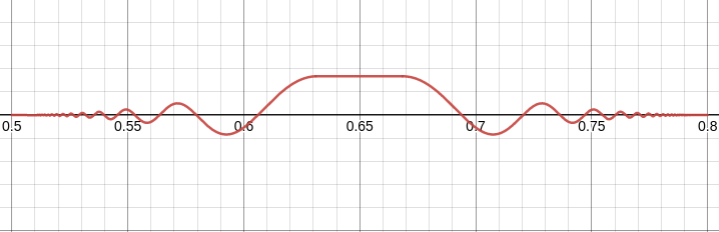
\includegraphics[scale=0.4]{img/volterra.png}
	\caption{Representation of $f_{0.5,0.8}$}
\end{figure}

Let us focus on the endpoint $a$ to gain some intuition about this function. 
It is obvious that this function is continuous at every point on $[a,b]$, but 
we will focus on the continuity at $a$. We see that $\forall x \in [a,b],
|f_{a,b}(x)| < (x-a)^2$. Thus by the squeeze theorem, we have that 
\begin{equation*}
	\lim_{x\rightarrow a^+} (x-a)^2 = 0 \implies \lim_{x\rightarrow a^+} f_{a,b}(x) = 0.
\end{equation*}
A similar argument holds for $b$ with the bound $\forall x\in [a,b], (b-x)^2$.

It is also important to observe that near the endpoints $a$ and $b$, the
derivative of this function behaves much like the derivative of 
$x^2\sin(\frac{1}{x})$. For example, near $a$ we have,
\begin{equation*}
	f'_{a,b}(x) = 2(x-a)\sin\bigg(\frac{1}{x-a}\bigg)
		-\cos\bigg(\frac{1}{x-a}\bigg).
\end{equation*}
Thus we have that there exists an epsilon neighborhood about
$a$ such that $f'_{a,b}$ oscillates infinitely between an upper bound of $1$ and
a lower bound of $-1$. This implies we have an essential discontinuity at $a$. 
A similar argument can be made for the endpoint $b$. In fact, the derivative
exists on the entire open interval $(a,b)$.

Finally, we observe that the derivative of this function on any interval is
bounded as follows:
\begin{equation*}
	|f'_{a,b}(x)| < 2(b-a)+1.
\end{equation*}
Now we are ready to define Volterra's function. We define Volterra's function 
$V:[0,1]\rightarrow \R$ as follows,
\begin{equation}
	V(x) = \begin{cases}
		f_{a,b}(x), & \text{if $x \in (a,b)$ for some interval $(a,b) \subset [0,1]\setminus \sF$ }\\
		0, & \text{if $x \in \sF$}
	\end{cases}.
\end{equation}

This next part is important. As we showed in the proof of proposition
\ref{prp:fat}, there no subinterval of $[0,1]$ is a subset of $\sF$. 
Thus, for every interval $(a,b) \subset [0,1] \setminus \sF$, the endpoints
$a,b$ are members of $\sF$. We have that $V$ is continuous on $[0,1]$.

\begin{figure}[H]
	\centering
	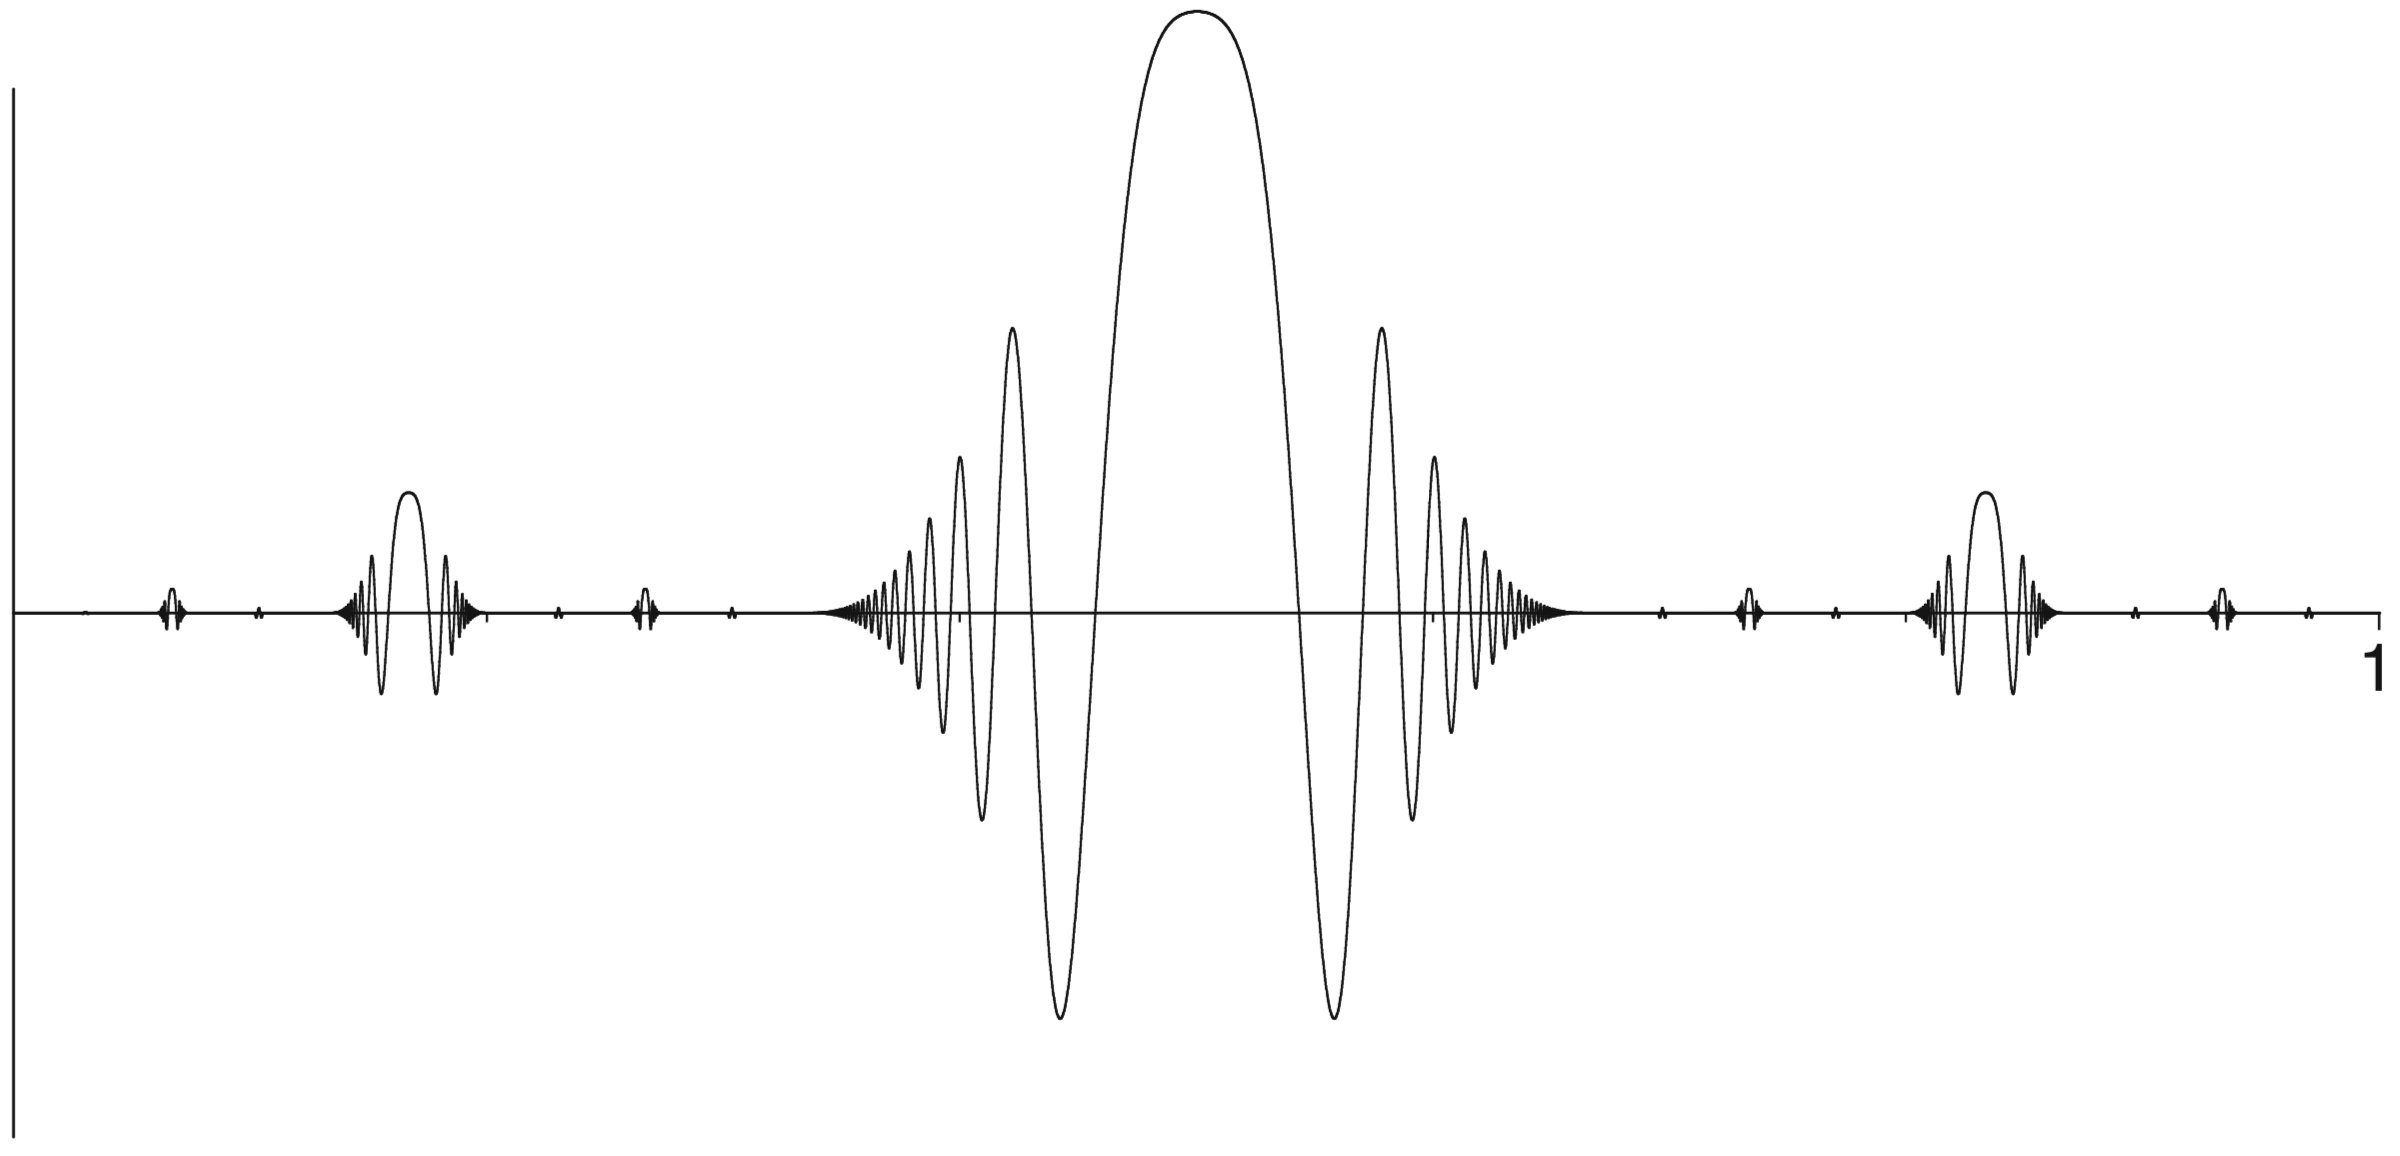
\includegraphics[width=\textwidth/2]{img/volterra-func.jpeg}
	\caption{Representation of $V$ on $[0,1]$}
	\tiny{Image Courtesy of Professor Dave Richeson}
\end{figure}

We also have that $V$ is differentiable on $[0,1]$. It is obvious that $x
\not \in \sF$ since $f_{a,b}$ is differentiable on any interval it is defined on. 
However, we need to show that it is differentiable for all points in $\sF$. We 
claim that for all elements in $\sF$, the derivative of $V$ is $0$.
\begin{prop}
	$\forall x \in \sF, V'(x) = 0$. 
\end{prop}
\begin{proof}
	We want to show that $\forall \epsilon > 0, \forall t \in [0,1], \forall x
	\in \sF, |t-x|<\epsilon \implies \frac{V(t) - V(x)}{t-x} = 0$. Let $\epsilon
	>0, t\in [0,1]$, and $x \in \sF$ be given. Suppose that $|x-t|<\epsilon$.
	We have two cases. 
	\begin{enumerate}
		\item Suppose $t \in \sF$. Then we have the following,
		\begin{equation*}
			\frac{V(t) - V(x)}{t-x} = \frac{0}{t-x} = 0.
		\end{equation*}
		\item Suppose $t \in \sF$. Then by definition, we have that 
		$t\in (a,b) \subset [0,1]\setminus \sF$. Without loss of generality,
		suppose that $a$ is the endpoint nearest to $x$. Then by definition
		of Volterra's function, we have,
		\begin{equation*}
			\frac{V(t) - V(x)}{t-x} = \frac{f(t)-0}{t-x} \leq \frac{f(t)}{t-a} <
			\frac{|t-a|^2}{|t-a|} = |t-a| < \epsilon.
		\end{equation*}
	\end{enumerate}
\end{proof}

Since the derivative at every point of the Volterra function has an oscillation 
similar to $\cos(\frac{1}{x})$ approaching from either the left, right, or
both, then the derivative at that point will be discontinuous. In other words,
the domain of discontinuity $D(V') = \sF$. As discussed earlier, $m(\sF) >0$,
thus by Lebesgue's criteria for Riemann integration, $\int_a^b V'(x)dx$ is not
defined.

\section{Lebesgue's Integral}
\begin{quote}
\textit{I have to pay a certain sum, which I have collected in my pocket. I take the
bills and coins out of my pocket and give them to the creditor in the order I
find them until I have reached the total sum. This is the Riemann integral. But
I can proceed differently. After I have taken all the money out of my pocket I
order the bills and coins according to identical values and then I pay the
several heaps one after the other to the creditor. This is my integral.}

\uppercase{\tiny{- Henri Lebesgue}}
\end{quote}

Finally, we arrive at Lebesgue's theory of integration. In his foundational
paper, Lebesgue introduces his integral with a simple yet brilliant
construction. Lebesgue begins,

\begin{quote}
	To define the integral of an increasing continuous function,
	\begin{equation*}
		y(x) (a\leq x \leq b)
	\end{equation*}
	We divide the interval $(a,b)$ into subintervals and sums the quantities
	obtained by multiplying the length of each subinterval by one of the values 
	of $y$ when $x$ is in the subinterval by one of the values. If $x$ is in
	the interval $(a_i,a_{i+1})$, $y$ varies between certain limits 
	$m_i$ and $m_{i+1},x$ is between $a_i$ and $a_{i+1}$$\cdots$Let the function 
	$y$ range between $m$ and $M$. Consider the situation
	\begin{equation*}
		m = m_0 < m_1 < m_2 < \ldots < m_{p-1} < M = m_p
	\end{equation*}
	$y =m$ when $x$ belongs to the set $E_0; m_{i-1}$ when $x$ belongs to the set
	$E_i$\footnote{Translator's Note: Without comment, he is defining $E_0 = y^{-1}(m) = \{x \in
	[a,b]: y(m) = m\}$, and each $E_i = y^{-1}(m_{i-1},m_i]$.}. We will define
	the measures $\lambda_0,\lambda_i$ of these sets. Let us consider one or the
	other of the two sums
	\begin{equation*}
		m_0\lambda_0+\sum m_i\lambda_i;
		m_0\lambda_0+\sum m_{i-1}\lambda_i;
	\end{equation*}
	\textit{If, when the maximum difference between two consecutive $m_i$ tends
	to zero, these sums tend to the same limit independent of the chosen $m_i$,
	this limit will be, by definition, the integral of $y$, which will be called
	integrable.}
\end{quote}

\subsection{Building Intuition}

Lebesgue's integral is fairly simple to define, yet upon first read it is hard 
to grasp what he is actually doing. On a more intuitive level, we can
understand Lebesgue's integral as a backwards  approach to the Riemann
integral--instead of partitioning the domain, we partition the range. However,
by this, we implicitly partition the domain! Here's another way to think about
it: when Riemann partitions the domain, he chooses what the width of each
rectangle will be, and the function determines the height for each rectangle. 
When Lebesgue partitions the range, he decides the height of the rectangle, 
then finds where on the function's domain the function allows him to build 
such rectangles.

Let's look at an example to drive this point home. Suppose that we wanted to
approximate the integral of the function $f(x) = 2-x^2$ on the interval
$[-\sqrt{2},\sqrt{2}]$. How would we do this using Lebesgue's approach?
Let's begin by partitioning the range into $4$ parts $\I_f = [0,2] =
[0,\frac{1}{2}) \cup [\frac{1}{2},1) \cup [1,\frac{3}{2}) \cup [\frac{3}{2},2]$.
Then we find the pre-image of partition. We have:
\begin{itemize}
	\item 
	$P_1 = f^{-1}([0,\frac{1}{2})) = [-\sqrt{2},-\sqrt{3/2} ) \cup (\sqrt{3/2},\sqrt{2}]$;
	\item 
	$P_2 = f^{-1}([\frac{1}{2},1))= [-\sqrt{3/2},-1) \cup (1,\sqrt{3/2}]$;
	\item 
	$P_3 = f^{-1}([1,\frac{3}{2})) = [-1,-1/\sqrt{2}) \cup (1/\sqrt{2},1]$;
	\item 
	$P_4 = f^{-1}([\frac{3}{2},2])= [-1/\sqrt{2},1/\sqrt{2}]$.
\end{itemize}

Observe that $P_1 \cup P_2 \cup P_3 \cup P_4 = \D_f$!
Now, like Riemann, we can approximate area by both upper and lower rectangles. 
Let the height of the upper rectangles be defined as $\sup(f(P_k))$ and the 
height of the lower rectangles be defined as $\inf(f(P_k))$. This gives
us the following,
\begin{itemize}
	\item $\inf(f(P_1)) = 0; \sup(f(P_1)) = \frac{1}{2}$.
	\item $\inf(f(P_2)) = \frac{1}{2}; \sup(f(P_2)) = 1$.
	\item $\inf(f(P_3)) = 1; \sup(f(P_3)) = \frac{3}{2}$.
	\item $\inf(f(P_4)) = \frac{3}{2}; \sup(f(P_4)) = 2$.
\end{itemize}

Here we finally realize why we spent so much time building up measure theory. 
We see that the pre-image of many of these intervals have breaks, so in order to
measure the ``width'' of all the rectangles with a certain height, we simply 
take the Lebesgue measure of pre-image! Since each $P_k$ is an interval or an
union of interval, we calculate the measure of each as follows.
\begin{itemize}
	\item $m(P_1) =  2(\sqrt{2} - \sqrt{3/2})$.
	\item $m(P_2) =  2(\sqrt{3/2} - 1)$.
	\item $m(P_3) =  2(1-\frac{1}{\sqrt{2}})$.
	\item $m(P_4) = \sqrt{2}$.
\end{itemize}
This gives use the following upper and lower sums:
\begin{equation*}
	S = \frac{1}{2}\cdot m(P_1) + 1\cdot m(P_2) + \frac{3}{2}\cdot m(P_3) + 2\cdot m(P_4)
	\approx 4.352,
\end{equation*}
\begin{equation*}
	s = 0\cdot m(P_1) + \frac{1}{2}\cdot m(P_2) + 1\cdot m(P_3) +
	\frac{3}{2}\cdot m(P_4) \approx 2.931.
\end{equation*}
Relating this back to Lebesgue's definition, we can see that as lengths of the 
range's partitions tend towards 0, our approximation will approach the actual area. 
In fact, because this function is so simple, we can calculate its integral
exactly. We have,
\begin{equation*}
	\int^{\sqrt{2}}_{-\sqrt{2}} 2-x^2 dx = 
		\bigg[2x - \frac{x^3}{3} \bigg]^{\sqrt{2}}_{-\sqrt{2}} = 
		\bigg(2(\sqrt{2}) - \frac{\sqrt{2}^3}{3} \bigg) - \bigg( 2(-\sqrt{2}) -
		\frac{(-\sqrt{2})^3}{3} \bigg) \approx 3.771.
\end{equation*}
Thus we can see that this Lebesgue approximation gives us a fairly decent bound on the 
actual value. 

\begin{figure}[H]
	\centering
	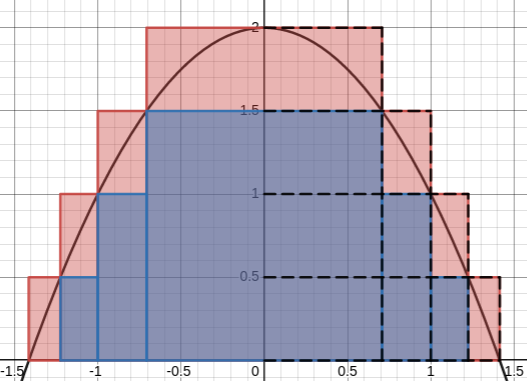
\includegraphics[scale=0.4]{img/approx.png}
	\caption{Lebesgue Approximation of $f(x) = 2-x^2$ with $4$ Range Partitions}
\end{figure}

After all of that, it is clear that performing a Riemann approximation would be
much easier. However, we are not interested in Lebesgue's integral for its 
computational ease. It is the theoretical advantages we are after. In fact, if
a function is Riemann integrable it is automatically Lebesgue integrable. This
fact can ease computational headaches.

\subsection{Integration of Simple Functions}

In order to get a better grasp on Lebesgue integration, it is best to start 
simple. We will introduce a class of simple functions that are easy to integrate
and build off them. 

\begin{definition}
	Let $A \subseteq \R$, we define the \textit{indicator function} of $A$
	as $\forall x \in \R$,
	\begin{equation}
		1_{A}(x) = \begin{cases}
			1 & \text{if  $x\in A$} \\	
			0 & \text{if $x\not \in A$} \\	
		\end{cases}.
	\end{equation}
\end{definition}

\begin{definition}
	Let $a_1,\cdots,a_k \in \R$ and the sets $A_1,\cdots,A_k \subset \R$ be 
	disjoint measurable sets with finite measure. We define an
	\textit{simple function} (SF) $f$ as any function that can be written in the
	form,
	\begin{equation}
		f = \sum_{i=1}^k a_i1_{A_i}.
	\end{equation}
\end{definition}

\begin{definition}
	The \textit{Lebesgue Integral} of an SF is $f:[a,b] \rightarrow \R$,
	\begin{equation}
		\int_{\R} f(x) dx \coloneqq \sum_{i=1}^k a_k m(A_k).
	\end{equation}
\end{definition}
Now that we have a definition, let's return to our old friend 
$1_{\Q}:[0,1] \rightarrow \{0,1\}$. What is the Lebesgue integral of this
function? Since $\Q\cap [0,1]$ is countable, we have that $m(\Q\cap [0,1]) = 0$, and since 
$1_{\Q}$ is an SF, we have that the integral of $1_{\Q}$ is,
\begin{equation*}
	\int_{[0,1]} 1_{\Q} = 1\cdot m(\Q\cap [0,1]) = 0.
\end{equation*}
We see that this simple application of the Lebesgue integral is able to deal
with functions that caused serious problems for Riemann's integral. The next
theorem outlines some of properties of SF.
\begin{theorem}
	Let $f,g$ be SF's and $c \in \R$. The following are true:
	\begin{enumerate}
	\item $cf$ is also an SF and
		\begin{equation}
			c\int f= \int cf.
		\end{equation}
	\item $f+g$ is also an SF and
		\begin{equation}
			\int f+g = \int f + \int g.
		\end{equation}
	\item $|f|$ is also an SF and
		\begin{equation}
			\bigg| \int f\bigg| = \int |f|.
		\end{equation}
	\item $f \leq g \implies \int f \leq \int g$ .
	\end{enumerate}
\end{theorem}

\subsection{Integration of Measurable Functions}

Now that we have established a theory of integration for SF, we can use these
facts to further generalize the Lebesgue integral to more general functions. 
Let us define how we can extend measure theory to functions. We define a 
non-negative measurable function as follows. 

\begin{definition}
	Let $E\subset \R$ be a measurable set and $f:E\rightarrow \bar{\R}$. We say $f$ is a 
	measurable function if $\forall \alpha \in \R, f^{-1}((\alpha,\infty])$ is measurable.
\end{definition}

\begin{theorem}
	Let $E \subset \R$ be a measurable set and $f:E \rightarrow \bar{\R}$. Then the
	following are equivalent:
	\begin{enumerate}
		\item $\forall \alpha \in \R, f^{-1}([\alpha,\infty])$ is measurable.
		\item $\forall \alpha \in \R, f^{-1}([-\infty,\alpha])$ is measurable.
	\end{enumerate}
\end{theorem}

\begin{definition}
	Let $f:\R \rightarrow \R$ be a non-negative measurable function. We define
	the Lebesgue integral of $f$ as,
	\begin{equation}
		\sup \bigg\{ \int g : g \text{ is an SF such that } 0 \leq g \leq f\bigg\}.
	\end{equation}
\end{definition}

In other words, for some non-negative measurable function, we are able to
approximate its integral with SF's from below, and the least upper bound
will be the integral of this function. Observe that $\int f = +\infty$ and 
$f$ may be an SF as well without conflict.

\begin{theorem}
	Let $f,g$ be non-negative measurable functions and $c \in \R^{+}$. The 
	following properties hold:
	\begin{enumerate}
		\item 
			\begin{equation}
				\int cf = c\cdot \int f.
			\end{equation}
		\item 
			\begin{equation}
				\int (f + g) = \int f + \int g
			\end{equation}
		\end{enumerate}
\end{theorem}

The proof for additivity of the Lebesgue integral is non-trivial. We will
need a squeeze theorem to help us along the way. This proof is taken from
Richard Beals' Real Analysis with some adjustments for clarity. Let's first look at the 
lemma.

\begin{lemma}
	Let $f$ be a bounded, measurable function and $A$ be a 
	set with finite measure. $\forall \epsilon > 0$, there exists SFs $f_1$ and $f_2$ such 
	that $f_1\leq f \leq f_2$ on $A$ and $\forall x \in \R, f_1 - f_2 \leq
	\epsilon$ .
\end{lemma}
\begin{proof}
	Let $\epsilon > 0$ be given.
	Choose an $M$ such that $\forall x \in \R, |f(x)| \leq M$ and partition the
	interval $[-M,M]$ into disjoint intervals $I_1,I_2,\ldots,I_n$ such that
	given any $I_k, |I_k| \leq \epsilon$. Let $A_k = A \cap f^{-1}(I_k)$. Given
	any $I_k$, let $a_k$ be its left end point and $b_k$ be its right endpoint.
	Define $f_1, f_2$ as,
	\begin{equation*}
		f_1 \coloneqq \sum^{n}_{k=1} a_k 1_{A_k},
		f_2 \coloneqq \sum^{n}_{k=1} b_k 1_{A_k}.
	\end{equation*}

	\begin{enumerate}
		\item 
		We want to show that $\forall x \in A, f_1(x) \leq f(x) \leq f_2(x)$.
		Let $x \in A$ be given, choose $I_k$ such that $x\in A_k$. Then we have
		that $f(x) \in I_k$. By choice of $f_1$ and $f_2$, we have that 
			\begin{equation*}
				f_1(x) = a_k \leq f(x) \leq b_k = f_2(x).
			\end{equation*}
		\item We want to show that $f_1 - f_2 \leq \epsilon$. We have that,
		\begin{equation*}
			f_1 - f_2 = \sum^{n}_{k=1} a_k 1_{A_k} - \sum^{n}_{k=1} b_k 1_{A_k}
				 =\sum^{n}_{k=1} (a_k - b_k) 1_{A_k}
				 =\sum^{n}_{k=1} |I_k|  1_{A_k}
				 \leq \sum^{n}_{k=1} \epsilon\cdot  1_{A_k}
		\end{equation*}
		Since each $I_k$ is disjoint, then given an $x \in A_k = A\cap f^{-1}(I_k)$,
		$x$ will be unique to that $A_k$, so only one of the indicator
		functions will evaluate to $1$ otherwise each $1_{A_k}$ will evaluate to
		$0$. This gives us $\forall x\in \R$,
		\begin{equation*}
			 \epsilon \cdot \sum^{n}_{k=1}  1_{A_k}(x) \leq \epsilon.
		\end{equation*}
	\end{enumerate}
\end{proof}

\begin{theorem}
	Let $f,g$ be bounded, non-negative, and measurable functions, then we have 
	$\int f + \int g = \int (g+f)$.
\end{theorem}
\begin{proof}
	Let $f_1,g_1$ both be SFs such that $0 \leq f_1 \leq f$ and 
	$0 \leq g_1 \leq g$. This gives us,
	\begin{equation*}
		\int f_1 + \int g_1 = \int (f_1 + g_1) \leq \int (f+g).
	\end{equation*}
	If we take the supremeum over all such possible SFs, we get the following
	\begin{equation*}
		\int f + \int g \leq \int (f+g).
	\end{equation*}
	The reverse inequality is less trivial. Let $h$ be a SF such that 
	$0\leq h \leq f+g$. Let $A$ be the set where $h >0$. We note that this
	set has finite measure and $h$ is bounded. Thus we have $h\land g$ and $h\land g$
	are both bounded. Using the lemma from above, choose SFs $f_1, g_1$ such 
	that,
	\begin{equation*}
		0 \leq f_1 \leq h \land f \leq f_1 +\epsilon, 
		0 \leq g_1 \leq h\land g \leq g_1+ \epsilon.
	\end{equation*}
	Because $h \leq f+g$, combining these inequalities gives us the following,
	\begin{equation*}
		h \leq (h \land f) + (h\land g) \leq f_1 + g_1+ 2\epsilon\cdot 1_A.
	\end{equation*}
	Thus we can construct the following inequality,
	\begin{equation*}
		\int h \leq \int f_1 + \int g_1 + 2\epsilon m(A) \leq \int f + \int g +
		2\epsilon m(A).
	\end{equation*}
	Next, we take the infimum over $\epsilon > 0$, and then take the supremum 
	over $h \leq f+g$ we get,
	\begin{equation*}
		\int (f+g) \leq \int f + \int g.
	\end{equation*}
\end{proof}

\subsection{Signed Measurable Functions}

Now that we have a working definition for non-negative measurable functions, we
need a way to handle negative measurable functions. We can do this by signing
the functions.

\begin{definition}
Let $f$ be a real-valued or extended-real-valued function defined on
the set $E$ such that $\forall x \in E$, 
\begin{equation}
	f^+(x) = \begin{cases}
		f(x) & \text{if $f(x) > 0$} \\
		0 & \text{otherwise} \\
	\end{cases}.
\end{equation}

\begin{equation}
	f^-(x) = \begin{cases}
		-f(x) & \text{if $f(x) < 0$}\\
		0 & \text{otherwise}
	\end{cases}.
\end{equation}
\end{definition}
It follows from the definition that these functions are measurable if $f$ is 
measurable, and we have:
\begin{equation}
	f = f^+ - f^-;	|f| = f^+ + f^-.
\end{equation}

\begin{definition}
	The signed function $f$ is said to be integrable if $\int |f| < +\infty$.
\end{definition}

This concludes our introduction of the basic definition and properties 
of Lebesgue's integral. Finally, we will move on to its two main theoretical
advantages over Riemann's integral.

\subsection{Dominated Convergence Theorem}

If we recall back to section \ref{sec:limitproblem} regarding the limit 
problem where we could define a sequence of bounded functions each of whom were
be Riemann integrable, yet the limit was not integrable. This reality raised 
the question: under what conditions can we move the limit inside of the
integral? Does Lebesgue's integral resolve this issue? The answer is somewhat.

First, we must dispense with the possibility that a sequence of
measurable functions could converge to a nonmeasurable function. Fortunately,
a convergent sequence of measurable functions will always converge pointwise to 
a measurable function. The following proof is again adapted from Richard Beals' 
Real Analysis.
\begin{theorem}
	Let $(f_n)^{\infty}_{n=1}$ be a sequence of measurable functions such that 
	$\forall x \in \R, \lim_{n\rightarrow \infty} f_n(x) = f(x)$, then $f$ is 
	measurable. 
\end{theorem}
\begin{proof}
	Let $\alpha, x \in \R$ be given. We want to show that  
	$x \in \{z \in \R : f(z) > \alpha\}$ is measurable. Suppose that $x \in \{z
	\in \R : f(z) > \alpha\}$. Then we can say for some $m \in \N, f(x) > \alpha+\frac{1}{m}$. Since 
	$f_n \rightarrow f$, there exists an $N \in \N$ such that 
	$\forall n \geq N, f_n(x) > \alpha+\frac{1}{m}$. This yields the following
	containment,
	\begin{equation*}
		\{z \in \R : f(z)  > \alpha \} \subset \bigcup^{\infty}_{m=1} \bigcup^{\infty}_{N=1} \bigcap^{\infty}_{n=N}
		\bigg\{z\in\R : f_n(z) > \alpha + \frac{1}{m}\bigg\}
	\end{equation*}
	Now suppose that $x$ is contained in the right hand set. Then for some 
	$m,N \in \N$, we have $\forall n \geq N, f_n (x) > \alpha + \frac{1}{m}$.
	Thus for the limit $f(x)$, we have,
	\begin{equation*}
		f(x) \geq \alpha + \frac{1}{m} > \alpha.
	\end{equation*}
	Therefore we have set equality and  $\{z \in \R : f(z) > \alpha\}$ is
	measurable. 
\end{proof}

This fact gives us the assurance that we will not converge to a function that
we cannot integrate given a sequence of integrable functions. However, it is
still not the case that we can always move the limit inside of the integral.
The following theorem is called Lebesgue's Dominated Convergence Theorem (DCT),
and is considered one of the greatest advantages of the Lebesgue integral over
the Riemann integral. 
\begin{theorem}[Dominated Convergence Theorem]
	Let $(f_n)^{\infty}_{n=1}$ be a sequence of measurable functions such that
	$\forall x \in \R, \lim_{n\rightarrow \infty}f_n(x) = f(x)$. Assume that
	$\forall n \in \N$ there exists an integrable function $g$ such that
	$\forall x \in \R, |f_n(x)| \leq g(x)$. Then,
	\begin{equation}
		\lim_{n\rightarrow \infty} \int f_n = \int f.
	\end{equation}
\end{theorem}

This theorem gives us precise conditions under which we can move the limit
inside the integral. Summarizing this theorem, it says: if we have a sequence of
measurable functions that converge to a measurable function, and that sequence
(including its limit) is \textit{dominated} pointwise by some function $g$,
then we can move the limit in. Of course, good mathematicians always ask, can we reduce our
assumptions? Unfortunately, we cannot strengthen this theorem. Next, we will go
over a simple example that illustrates why we cannot strengthen this theorem.

Let us define a simple sequence of functions $f_n: [0,1] \rightarrow \R$ such
that $\forall n \in \N, \forall x \in \R$, 
\begin{equation*}
	f_n(x) = n \cdot 1_{(0,\frac{1}{n})}(x).
\end{equation*}
We see as $n \rightarrow \infty$ that this function cannot be dominated. In
fact suppose that could be.
\begin{proof}
Assume towards contradiction that there is some $g: \R \rightarrow \R$ such that
$\forall n \in \N, \forall x \in \R, |f_n(x)| \leq g(x)$. Then, choose an 
$n \in \N$ such that $n > \sup(g[0,1])$, and choose $x \in (0,\frac{1}{n})$. 
We have:
\begin{equation*}
	|f_n(x)| = |n\cdot 1_{(0,\frac{1}{n})}(x)| = n > g(x).
\end{equation*}
Contradiction.
\end{proof}

Thus we see that this function does not satisfy the dominated hypothesis in
the DCT. The next natural question is what is the limit of this sequence? We
claim that this sequence approaches the 0 function.
\begin{prop}
	$\forall x \in [0,1], \lim_{n\rightarrow \infty} f_n(x) = \bold{0}(x)$.
\end{prop}
\begin{proof}
	Let $x \in [0,1]$ be given. We have exactly two cases. 
	\begin{enumerate}
		\item Assume that $x = 0$. Then $\forall n \in \N, f_n(x) = 0$.
		\item Assume that $x\neq 0$. Let $\epsilon > 0, n\in \N$ be given.
		Choose $N \in \N$ such that $\frac{1}{N} <x$. Assume that $n \geq N$.
		Then we have,
		\begin{equation*}
			|f_n(x) - 0| = |n\cdot 1_{(0,\frac{1}{n})}(x)|  = 0 < \epsilon.
		\end{equation*}
	\end{enumerate}
\end{proof}

Now, let us evaluate both sides of the equality of the DCT and see if it holds. 
For the left hand side we have,
\begin{equation*}
	\lim_{n\rightarrow \infty} \int_{[0,1]} f_n(x) dx = 
	\lim_{n\rightarrow \infty} n\cdot \frac{1}{n} = 1.
\end{equation*}
and for the right hand side we have,
\begin{equation*}
	\int_{[0,1]} \lim_{n\rightarrow \infty} f_n(x) dx = 
	\int_{[0,1]} \bold{0}(x) dx = 0.
\end{equation*}
Therefore we see that it is not possible to move the limit inside of the
integral, and we conclude that we cannot remove this condition. 
Even though we cannot remove this condition, because it is so mild, the DCT is 
an extremely powerful tool to have.

\subsection{Lebesgue's Fundamental Theorem of Calculus}

The final major issue that Lebesgue's integral addresses is the anti-derivative
problem. After all, this was Lebesgue's primary goal. Lebesgue's 
integral gives us a precise condition for which functions satisfy the FTC. It 
involves a stricter notion of continuity called absolute continuity. We define 
it as follows.
\begin{definition}
	Let $[a,b] \subset \R$ and $f:[a,b] \rightarrow \R$, we say that $f$ is 
	\textit{absolutely continuous} if $\forall \epsilon  > 0$, $\exists \delta
	>0$, such that when a sequence of pairwise disjoint subintervals $(x_k,y_k)$
	for $x_k < y_k \in [a,b]$ satisfies:
	\begin{equation}
		\sum_{k} (x_k - y_k) < \delta \implies \sum_{k} |f(x_k) - f(y_k) | < \epsilon.
	\end{equation}
\end{definition}

The next theorem is Lebesgue's Fundamental Theorem of Calculus.
\begin{theorem}[Lebesgue's Fundamental Theory of Calculus]
	Let $f:[a,b] \rightarrow \R$ be absolutely continuous on $[a,b]$, 
	then,
	\begin{equation}
		\int_{[a,b]} f'(x) dx = f(b) - f(a).
	\end{equation}
\end{theorem}
Unfortunately, deeper investigation into why such functions have this property is
beyond the scope of this paper.\footnote{For a detailed proof see \cite{pouso:2012}}
The key take away is that Lebesgue's theory of 
integration provides us with a clear context in which we can apply 
the FTC to a given function. Ultimately, Lebesgue's integral puts the theory of 
integration on firm theoretical ground and addresses many of the theoretical 
concerns prior to its introduction.

\newpage
\bibliography{refs}

\end{document}
